%% fsm-stackelberg — manuscript draft (cas-sc)
%% Compile: latexmk -pdf manuscript.tex  (run inside els-cas-templates/)

\PassOptionsToPackage{hyperfootnotes=false}{hyperref}
\documentclass[a4paper,fleqn]{cas-sc}

\usepackage{amssymb}
\usepackage{amsmath}
\usepackage{graphicx}
\usepackage{booktabs}
\usepackage{tabularx}
\usepackage[authoryear,longnamesfirst]{natbib}
\usepackage{multirow}
\usepackage{algorithm}
\usepackage{algpseudocodex}
\usepackage{xcolor}
\usepackage[most]{tcolorbox}

\graphicspath{{figs/}{../figures/}}

%% Semi-formal proposition box (avoids depending on a theorem environment).
\newtcolorbox{propbox}[1][]{enhanced,breakable,
  colback=blue!2,colframe=blue!45,boxrule=0.4pt,arc=3pt,
  left=8pt,right=8pt,top=5pt,bottom=5pt,
  fonttitle=\bfseries,coltitle=black,title=Proposition,#1}

\newcommand{\Ecal}{\mathcal{E}}
\newcommand{\Acal}{\mathcal{A}}
\newcommand{\Qcal}{\mathcal{Q}}
\newcommand{\Scal}{\mathcal{S}}
\newcommand{\tri}{\triangleright}

\begin{document}

\shorttitle{Stackelberg Diagnosis--Repair for LLM-Based ECR}
\shortauthors{Peng et al.}

\title[mode=title]{A Stackelberg Inspection Game for Diagnosis--Repair in LLM-Based Empty Container Repositioning Optimization}

\author[dlmu]{Kangzhen Peng}
\ead{pengkangzhen@dlmu.edu.cn}

\author[dlmu]{Siqi Duan}
\ead{duansiqi@dlmu.edu.cn}

\author[nbu]{Yuhong Wang}
\ead{wangyuhong@nbu.edu.cn}

\author[lnut]{Jiaxin Cai}
\ead{jgcaijx@lnut.edu.cn}

\author[djtu]{Shida Xu}
\ead{xushida@djtu.edu.cn}

\author[dlmu]{Zhihong Jin\corref{cor1}}
\ead{jinzhihong@dlmu.edu.cn}
\ead[url]{https://orcid.org/0000-0003-4342-1561}

\cortext[cor1]{Corresponding author.}

\affiliation[dlmu]{organization={College of Transportation Engineering, Dalian Maritime University},
  addressline={No. 1 Linghai Road}, city={Dalian}, postcode={116026}, state={Liaoning}, country={China}}
\affiliation[nbu]{organization={Faculty of Maritime and Transportation, Ningbo University},
  addressline={No. 169, Qixing South Road}, city={Ningbo}, postcode={315211}, state={Ningbo}, country={China}}
\affiliation[lnut]{organization={School of Economics and Management, Liaoning University of Technology},
  addressline={}, city={Jinzhou}, postcode={121001}, state={Liaoning}, country={China}}
\affiliation[djtu]{organization={College of Economics and Management, Dalian Jiaotong University},
  addressline={}, city={Dalian}, postcode={116028}, state={Liaoning}, country={China}}

\begin{abstract}
We recast the error diagnosis and repair stage of an LLM multi-agent
pipeline for Empty Container Repositioning (ECR) optimization as a Stackelberg
\emph{inspection game} defined on a state machine. A LangGraph finite-state machine orchestrates role-specialized
agents (Data Engineer $\to$ Model Expert $\to$ Python Developer $\to$ Solver)
and serves as the stage-game apparatus. When a solve fails, the diagnosis
agent acts as an \emph{inspector} (the Stackelberg leader) that commits, first
and observably, to an inspection policy: an evidence-ranked probing order
together with \emph{executed refutation} --- verifying every response by a
real re-solve rather than by cheap talk. The accused agents are
\emph{inspectees} (the followers): because a downstream layer is routinely
implicated by an upstream defect it did not cause, each accused agent has a
genuine private incentive to deflect blame, so its interests are not aligned
with truthful attribution. We formalize the mechanism and state a proposition
linking committed inspection to a reduced viable root-cause set, then test it
on a \emph{demand-uncertainty} sea--land ECR problem formulated as a two-stage
stochastic linear program: three fault plants (one per layer), three problem
instances, five diagnosis protocols, and shared frozen failure blackboards.
The measured mechanism is precise: probing is bound to the committed
order, so first-probe naming is exactly the ranking's alignment --- which
holds on every model-layer board and fails only for rank-invisible
semantic data faults --- while on the main grid only $14$ of the $30$
aligned first probes are confirmed by the round-one re-solve ($9$
overturned repairs, $7$ attributions stolen by downstream regeneration),
and a misaligned probe can conversely absorb an upstream fault outright;
causal commitment dominates single-judge, debate, and
reflexion naming (paired across all thirty shared boards without a single
discordance) at the lowest token cost, the
guilty layer complies at first contact under commitment (the rare
deflections observed all sit in non-committed arms and follow an
overturned repair), and $43$--$71\%$ of complying
repairs are overturned by the re-solve --- executed verification, not talk,
carries attribution. The order advantage replicates conditionally on the
ranking's ability to see the fault layer; for rank-invisible semantic data
faults we register a design revision rather than a post-hoc fix.
\end{abstract}

\begin{highlights}
\item Diagnosis--repair is cast as a Stackelberg inspection game defined on a LangGraph state machine as the stage-game apparatus.
\item The inspector commits, first-mover, to an evidence-ranked probing policy with executed refutation of every repair by re-solve.
\item Probing is bound to the committed order, so first-probe naming equals the ranking's alignment; round-one confirmation is separately gated by the repair passing the re-solve.
\item Committed inspection dominates single-judge, debate, and reflexion naming at the lowest token cost; guilty layers comply at first contact under commitment, and the rare deflections observed (all in non-committed arms) follow an overturned repair.
\end{highlights}

\begin{keywords}
\sep large language model
\sep multi-agent system
\sep Stackelberg game
\sep finite-state machine
\sep automated optimization modeling
\sep empty container repositioning
\end{keywords}

\maketitle

%==============================================================================
\section{Introduction}
\label{sec:intro}

Empty Container Repositioning (ECR) is a standing cost center in global
liner shipping. Trade imbalance leaves empty equipment stranded at import
hubs while export regions face shortages; planners must move empties across
sea and inland networks under capacity, transit-time, and inventory
limits~\citep{poiani2024ecr,wang2025ecrslot}. Under demand uncertainty the
problem is naturally a multi-stage (often two-stage) stochastic program:
first-stage repositioning commitments are made before scenario-dependent
export demand realizes, and recourse actions (e.g.\ leasing or spill) absorb
residual imbalance~\citep{poiani2024ecr,cai2025ecrjoint}. Building a
correct model therefore requires scarce domain expertise: admissible
sea--dry topologies, mode-specific costs, scenario trees or deterministic
equivalents, and recourse design that remains relatively complete. Small
misspecifications in data, mathematics, or solver code routinely yield
infeasible, suboptimal, or operationally meaningless plans.

Traditional practice addresses ECR with expert-built mixed-integer or
stochastic programs, meta-heuristics, and, more recently, multi-agent
reinforcement learning for joint repositioning and fleet
decisions~\citep{poiani2024ecr,cai2025ecrjoint}. These methods can be
strong once a model exists, but they share a structural bottleneck: every
new network, planning window, or uncertainty description must be
\emph{hand-modeled} by OR specialists. Reformulation is slow; knowledge is
hard to transfer across carriers; and the gap between how operations are
described in language and how they appear in an LP remains human-mediated.
Learning-based controllers alleviate online decision load but still
presume a correctly engineered state, action, and reward interface. In
short, the limiting resource is often not the solver, but the modeling
labor that feeds it.

Large language models (LLMs) change that interface. They parse
operational narratives and structured tables, propose mathematical
formulations, emit executable solver code, and iterate against tool
feedback~\citep{xiao2023coe,ahmaditeshnizi2024optimus}. These abilities
align with ECR pain points: the input is already a mixture of natural
language and instance data; the desired output is a compilable,
solvable model whose quality can be checked by an industrial MIP solver
and, when available, by a known optimum $z^{\star}$. Multi-agent
scaffolds (role-specialized data, modeling, and coding agents coordinated
by a shared state) further match the layered work of OR practice, from
data preparation through formulation to
implementation~\citep{wu2024autogen,xiao2023coe,ahmaditeshnizi2024optimus}.
Recent
maritime applications already use LLM agents for stowage-related planning
and sketch agent-based transportation modeling~\citep{liu2025llmtransport},
indicating that the same automation path is opening for container
logistics.

Automation, however, relocates rather than removes the reliability
problem. In a natural-language optimization (NLO) pipeline, defects
propagate along \emph{data $\tri$ model $\tri$ code}: an upstream modeling
error often surfaces as a downstream crash or wrong objective, so stack
traces mark the symptom locus rather than the certified root cause. Without
domain knowledge the pipeline cannot formulate ECR correctly in the first
place; with knowledge, failed solves still demand
\emph{attribution and repair}. Existing agentic OR systems rely mainly on
single-judge accusation, sequential backward repair, multi-agent
debate, or verbal reflection~\citep{du2023improving,shinn2023reflexion,liang2024mad}.
These protocols increase deliberation but treat diagnosis as (multi-call)
classification with cheap-talk self-checks. They do not commit an observable
inspection policy, do not verify accused replies by executed re-solve as a
discipline, and do not account for the private incentive of an innocent
downstream layer to deflect blame.

\paragraph{Thesis.}
We argue that diagnosis--repair under layered ECR modeling errors is a
Stackelberg~\citep{stackelberg1952} \emph{inspection
game}~\citep{avenhaus2002inspection,maschler1966inspection}.
A diagnosis agent acts as inspector (leader) and commits, first and
observably, to a policy $\sigma=(\omega,\nu)$: a probing order $\omega$
aligned with causal dependence, and a verification rule $\nu$ of
\emph{executed refutation} (a real re-solve under a strict-success test
against $z^{\star}$). Accused data, model, and code agents are inspectees
(followers) that choose to comply-and-repair or to deflect. Commitment
gives the mechanism teeth: a guilty layer's best response is to repair; an
innocent layer's deflection is upheld only if re-solve confirms it. We
instantiate the game on a LangGraph state machine as stage-game apparatus
and validate it on a demand-uncertainty sea--land ECR two-stage DEP
(Section~\ref{sec:ecr_model}).

\paragraph{Contributions.}
(i)~We cast diagnosis--repair in an LLM multi-agent NLO pipeline as a
Stackelberg inspection game on a finite-state machine.
(ii)~We specify an inspector commitment to causal-order probing with
executed refutation, inducing verifiable attribution rather than
confidence-routed accusation.
(iii)~We state a proposition that, under explicit premises on causal
layering and repair-path behaviour, causal-order inspection strictly
reduces the viable root-cause set relative to single-judge play without
dropping the true layer, and test it with commitment-order ablations and
baselines on demand-uncertainty ECR.
(iv)~We separate progressive domain-knowledge injection (necessary for ECR
solvability) from the game-theoretic diagnosis claim (necessary for
auditable repair).

Section~\ref{sec:related} reviews ECR research and the shift to agentic
NLO. Section~\ref{sec:ecr_model} gives the ECR problem description and
mathematical formulation.
Section~\ref{sec:method} develops the inspection mechanism.
Section~\ref{sec:experiments} reports the experimental campaign and
results; Section~\ref{sec:conclusion} concludes.

%==============================================================================
\section{Related Work}
\label{sec:related}

\subsection{Empty container repositioning}
\label{sec:related_ecr}
ECR has long been studied as a network optimization problem driven by
directional trade imbalance. Classical and contemporary OR formulations
use deterministic or stochastic mathematical programs for repositioning,
inventory, slot allocation, and related fleet decisions, often solved by
exact methods or meta-heuristics~\citep{wang2025ecrslot,cai2025ecrjoint}.
Under uncertainty and operational black-box constraints, configurable
partially observable models and two-stage learning procedures have been
proposed for joint repositioning and fleet
deployment~\citep{poiani2024ecr}. These lines establish ECR as a hard,
domain-rich benchmark with verifiable optima once a model is fixed. They
do not automate the passage from an operational description to that model.
Emerging LLM-agent work in maritime and transportation systems (e.g.\
text-to-stowage pipelines and conceptual LLM-agent transportation
frameworks)~\citep{liu2025llmtransport} suggests that natural-language
interfaces are becoming plausible for container logistics, but reliability
of the modeling--coding--solving chain remains open. We therefore use
demand-uncertainty ECR as a \emph{validation bed} with an expert DEP
optimum $z^{\star}$, not as a claim of a new ECR theory.

\subsection{From expert modeling to agentic natural-language optimization}
\label{sec:related_nlo}
The broader OR+LLM literature is shifting how optimization problems are
produced and checked. Chain-of-Experts orchestrates role-specialized agents
with forward construction and backward reflection for complex OR
tasks~\citep{xiao2023coe}; OptiMUS modularizes formulation, coding, and
evaluation against solver feedback at
scale~\citep{ahmaditeshnizi2024optimus,ahmaditeshnizi2024optimus03};
related expert-guided reasoning pipelines further target automated
optimization modeling~\citep{yang2025orthought}. Relative to classical
``expert writes the math, solver optimizes,'' this body of work exhibits
three coupled shifts. First, the \emph{object of study} moves from solving
a given mathematical program to turning unstructured descriptions and data
into a solvable, correct model. Second, \emph{verification} moves from
textual resemblance or manual reading toward executable checks (compile,
solve, and comparison to $z^{\star}$ when available), so success is judged
by whether the artifact passes a solver rather than by whether the prose
looks right. Third, once modeling is a multi-stage pipeline, \emph{reliability}
becomes first-class: errors cascade along data, model, and code; the failure
surface is often downstream of the true root cause. Domain knowledge
injection is necessary for problems such as ECR to be formulable at all;
failure attribution and diagnosis--repair are necessary for the pipeline to
recover when it does not. Our work sits in this third shift while retaining
executable solver verification as the hard truth signal.

\subsection{Reliability mechanisms in LLM multi-agent systems}
\label{sec:related_reliability}
Layered LLM multi-agent systems face a distinctive reliability problem:
errors cascade across role boundaries, and the observable failure surface
(crash, infeasibility, or wrong objective) is often downstream of the true
root cause. In NLO pipelines this appears as data~$\tri$~model~$\tri$~code
dependence---a modeling mistake may surface as a coding crash or a wrong
solve. Domain knowledge and role scaffolding are a \emph{prerequisite} for
hard OR tasks to be formulable at
all~\citep{wu2024autogen,xiao2023coe,ahmaditeshnizi2024optimus}, but they do
not by themselves certify which layer failed or compel a correct repair. A
complementary line therefore treats verification as executable rather than
textual: compile, solve, and check against solver feedback or a known
optimum when
available~\citep{ahmaditeshnizi2024optimus,ahmaditeshnizi2024optimus03}.
Two further mechanism families address post-failure recovery. Failure
attribution asks which agent and which step caused the failure: Who\&When
shows that even strong LLM judges remain far from reliable step-level
attribution~\citep{zhang2025whowhen}; subsequent work stresses full-trace
observability~\citep{chen2026traceelephant}, hierarchical or causal-graph
attribution~\citep{wang2026chief}, and Causal Agent Replay that intervenes
on trajectory steps and re-executes forward~\citep{shah2026car}.
Diagnosis--repair and multi-call protocols then try to act on that judgment:
single-judge accusation with status-based priors, reverse-order sequential
repair, multi-agent debate~\citep{du2023improving,liang2024mad}, and
Reflexion-style verbal memory~\citep{shinn2023reflexion}. These lines
increase deliberation or observability, yet they typically stop at naming
(or reflective re-prompting). Missing for layered OR pipelines is a
\emph{committed} inspection policy whose replies are settled by re-solve
under a strict success rule---the incentive-compatible, executed-refutation
mechanism we develop as a Stackelberg inspection game in
Section~\ref{sec:related_game}.

\subsection{Game-theoretic multi-agent LLM systems}
\label{sec:related_game}
Game-theoretic views of LLM multi-agent systems cover debate, Nash-style
coordination, and Stackelberg resource
governance~\citep{yi2025econ,stackelberg2026resource,du2023improving}.
Classical inspection games analyze an inspector who commits to a monitoring
policy and an inspectee who best-responds~\citep{avenhaus2002inspection,maschler1966inspection}.
In AI, the same leader-commitment logic underpins deployed Stackelberg
security games, where a defender commits to a randomized patrolling or
scheduling policy and adversaries best-respond after
surveillance~\citep{korzhyk2011security,tambe2011security}.
We use that template for layered NLO diagnosis--repair: the diagnosis agent
is the inspector; data/model/code agents are inspectees; commitment is to
causal-order probing plus executed refutation on the ECR blackboard. This
differs from resource Stackelberg controllers (token or tool budgets) and
from debate equilibria (message-passing agreement) in both players and
payoffs. The empirical spine is whether committed causal order improves
\emph{verifiable} attribution relative to unordered commitment and to
non-committed single-judge or multi-call baselines
(Section~\ref{sec:experiments}).

%==============================================================================
\section{Problem Description and Mathematical Formulation}
\label{sec:ecr_model}

\subsection{Problem description}
\label{sec:ecr_desc}
\label{sec:ecr_network}

We validate the diagnosis--repair mechanism on a sea--land Empty Container
Repositioning (ECR) problem under \emph{export-demand uncertainty}. The
application model is a two-stage stochastic linear program on a weekly
planning window (deterministic equivalent / DEP), adapted from our companion
formulation for demand-uncertainty ECR. Unlike the MAKO baseline's
deterministic shipper--consignee multi-commodity flow, the present benchmark
retains only sea and dry ports, treats empty supply as exogenous, and places
all randomness in scenario-dependent export demand. Agents in the pipeline
must formulate and solve this DEP from a natural-language description plus
structured instance data; the expert DEP optimum supplies the
strict-success rule used by the diagnosis mechanism
(Section~\ref{sec:stackelberg}).

The network is a directed multigraph on node set
$\mathcal{N}=\mathcal{H}\sqcup\mathcal{L}$, where sea ports
$\mathcal{H}=\mathcal{H}^{\mathrm{hub}}\sqcup\mathcal{H}^{\mathrm{spoke}}$
partition into global hubs and regional spokes, and $\mathcal{L}$ is the set
of dry ports. Inland moves use modes $\kappa\in\mathcal{K}$ (road, rail).
Rather than writing Big-M hinterland restrictions inside the LP, we
\emph{compile} topology into an admissible arc set
\begin{equation}
\mathcal{A}
\subseteq
\mathcal{N}\times\mathcal{N}\times\mathcal{K},
\label{eq:arc-set}
\end{equation}
built once from hinterland indicators $\lambda_{ij}$: include sea--dry arcs
$(i,j,\kappa)$ and $(j,i,\kappa)$ iff $\lambda_{ij}=1$, and dry--dry arcs
$(j_1,j_2,\kappa)$ iff $j_1$ and $j_2$ share a common hinterland sea port.
Each arc $a=(i,j,\kappa)\in\mathcal{A}$ carries transit time
$\tau_a$, unit repositioning cost $c_a^{\mathrm{repo}}$, and capacity
$F_a^{\mathrm{cap}}$. Flow variables exist only on $\mathcal{A}$;
inadmissible hinterland pairs simply never appear.

Time is discrete by week. Empty containers held at sea or dry ports serve
export demand. The empty supply $\xi_{n,t}$ at node $n$ in week $t$ is an
\emph{exogenous deterministic} parameter (no laden-to-empty conversion
dynamics). The core uncertainty is the scenario-dependent export demand
$\eta_{n,t}^{\omega}$ for $\omega\in\Omega$ with probabilities $\pi_{\omega}$.
Leasing is unbounded (at a premium); a heavily penalized spill variable
ensures relatively complete recourse under storage caps.

A full operational system may wrap successive windows in a rolling horizon.
For the agentic modeling task we fix a single window
$\mathcal{T}=\{1,\dots,H\}$ (smoke instance: $H{=}4$, $|\Omega|{=}5$) and ask
the pipeline to build the extensive-form DEP of the two-stage program below.
All decisions are continuous nonnegative TEUs; at weekly scale the integrality
gap is negligible.

\subsection{Mathematical formulation}
\label{sec:ecr_formulation}

\subsubsection{Sets, parameters, and variables}
\label{sec:ecr_notation}

\paragraph{Sets.}
$\mathcal{H}^{\mathrm{hub}}$, $\mathcal{H}^{\mathrm{spoke}}$, $\mathcal{L}$;
$\mathcal{N}^{\mathrm{inv}}=\mathcal{H}\cup\mathcal{L}$;
modes $\mathcal{K}$; admissible arcs $\mathcal{A}$ as in~\eqref{eq:arc-set};
scenarios $\Omega$; window $\mathcal{T}$.
For each node $n\in\mathcal{N}$ define the forward and backward stars
\begin{equation}
\mathcal{A}_n^{+}
=\{(n,j,\kappa)\in\mathcal{A}\},
\qquad
\mathcal{A}_n^{-}
=\{(i,n,\kappa)\in\mathcal{A}\}.
\label{eq:star-sets}
\end{equation}
Flow variables are indexed on arcs $(i,j,\kappa)\in\mathcal{A}$;
we write $x_{ij\kappa,t}^{\omega}$ interchangeably with $x_{a,t}^{\omega}$ for
$a=(i,j,\kappa)$.

\paragraph{Deterministic parameters.}
Exogenous supply $\xi_{n,t}$; spoke top-up $E_{i,t}$; initial inventory
$I_{n,0}$; committed inland arrivals $\bar{Q}_{n,t}^{\mathrm{arr}}$ (zero on the
first-window smoke instance); hub vessel calls $V_{i,t}\in\{0,1\}$ and
per-call bounds $B_i^{\mathrm{in}}$, $B_i^{\mathrm{out}}$; effective external
export floor
$\tilde{D}_{i,t}^{\mathrm{ext}}=\min\{D_{i,t}^{\mathrm{ext}},B_i^{\mathrm{out}}\}$;
per-arc $(\tau_{ij\kappa},c_{ij\kappa}^{\mathrm{repo}},F_{ij\kappa}^{\mathrm{cap}})$
for $(i,j,\kappa)\in\mathcal{A}$; storage caps $U_n^{\mathrm{cap}}$; sea costs
$c^{\mathrm{sea,in}}$, $c^{\mathrm{sea,out}}$; repositioning / holding / leasing /
spill costs $c_{ij\kappa}^{\mathrm{repo}}$, $c_n^{\mathrm{hold}}$,
$c_n^{\mathrm{lease}}$, $c^{\mathrm{spill}}$, with
$c^{\mathrm{spill}}\gg\max\{c_n^{\mathrm{lease}},c_n^{\mathrm{hold}},
c_{ij\kappa}^{\mathrm{repo}}\}$.

\paragraph{Random parameters.}
Demand $\eta_{n,t}^{\omega}$ and probabilities $\pi_{\omega}$
($\sum_{\omega}\pi_{\omega}=1$). Scenarios are drawn by truncated-normal
additive shocks about nominal means $\bar{\eta}_{n,t}$.

\paragraph{First-stage decisions (here-and-now).}
$y_{i,t}^{\mathrm{in}},\,y_{i,t}^{\mathrm{out}}\in\mathbb{R}_+$ for
$i\in\mathcal{H}^{\mathrm{hub}}$, $t\in\mathcal{T}$: hub sea arrivals
(arrival-week accounting) and departures, chosen \emph{before} demand is
revealed.

\paragraph{Second-stage decisions (wait-and-see).}
For each $\omega\in\Omega$: arc flows $x_{ij\kappa,t}^{\omega}$
($(i,j,\kappa)\in\mathcal{A}$), inventories $I_{n,t}^{\omega}$, leases
$r_{n,t}^{\omega}$, and spill $s_{n,t}^{\omega}$, all in $\mathbb{R}_+$.

\subsubsection{Mathematical model}
\label{sec:ecr_mathmodel}

The inland submodel is a \emph{node--arc} network formulation on the
admissible digraph $(\mathcal{N},\mathcal{A})$: topology is encoded by the
stars~\eqref{eq:star-sets}, and conservation at each node is written with
incidence sums over $\mathcal{A}_n^{\pm}$.

\paragraph{Stage~1 master problem [D1].}
\begin{align}
\min_{\boldsymbol{y}}\;
& \sum_{t\in\mathcal{T}}\sum_{i\in\mathcal{H}^{\mathrm{hub}}}
\bigl(c^{\mathrm{sea,in}} y_{i,t}^{\mathrm{in}}
+ c^{\mathrm{sea,out}} y_{i,t}^{\mathrm{out}}\bigr)
+ \sum_{\omega\in\Omega}\pi_{\omega}\,\Theta^{\mathrm{D}}(\boldsymbol{y},\omega)
\label{eq:d1-obj} \\
\text{s.t.}\;
& y_{i,t}^{\mathrm{in}} \le B_i^{\mathrm{in}} V_{i,t},
\quad \forall i\in\mathcal{H}^{\mathrm{hub}},\; t\in\mathcal{T},
\label{eq:d1-capin} \\
& y_{i,t}^{\mathrm{out}} \le B_i^{\mathrm{out}} V_{i,t},
\quad \forall i\in\mathcal{H}^{\mathrm{hub}},\; t\in\mathcal{T},
\label{eq:d1-capout} \\
& y_{i,t}^{\mathrm{out}} \ge \tilde{D}_{i,t}^{\mathrm{ext}} V_{i,t},
\quad \forall i\in\mathcal{H}^{\mathrm{hub}},\; t\in\mathcal{T},
\label{eq:d1-export} \\
& y_{i,t}^{\mathrm{in}},\; y_{i,t}^{\mathrm{out}} \ge 0.
\label{eq:d1-nn}
\end{align}

\paragraph{Stage~2 recourse [D2].}
Given $\boldsymbol{y}$ and realized $\eta^{\omega}$, write the node--arc
inflow and outflow through the stars~\eqref{eq:star-sets} as
\begin{equation}
\begin{aligned}
\mathrm{In}_{n,t}^{\omega}
&=\sum_{(i,n,\kappa)\in\mathcal{A}_n^{-}}
  x_{in\kappa,\,t-\tau_{in\kappa}}^{\omega},
\\
\mathrm{Out}_{n,t}^{\omega}
&=\sum_{(n,j,\kappa)\in\mathcal{A}_n^{+}}
  x_{nj\kappa,t}^{\omega},
\end{aligned}
\label{eq:d2-inout}
\end{equation}
with the convention $x_{ij\kappa,s}^{\omega}:=0$ if $s\notin\mathcal{T}$
(lagged arrivals outside the window enter via $\bar{Q}_{n,t}^{\mathrm{arr}}$).
The recourse problem is
\begin{equation}
\Theta^{\mathrm{D}}(\boldsymbol{y},\omega)
=\min_{\boldsymbol{x},\boldsymbol{I},\boldsymbol{r},\boldsymbol{s}}
\Bigl(
C^{\mathrm{repo}}(\omega)
+C^{\mathrm{hold}}(\omega)
+C^{\mathrm{lease}}(\omega)
+C^{\mathrm{spill}}(\omega)
\Bigr),
\label{eq:d2-obj}
\end{equation}
where the four activity cost blocks (repositioning / holding / leasing / spill)
are
\begin{align}
C^{\mathrm{repo}}(\omega)
&=\sum_{t\in\mathcal{T}}
  \sum_{(i,j,\kappa)\in\mathcal{A}}
  c_{ij\kappa}^{\mathrm{repo}}\,x_{ij\kappa,t}^{\omega},
\label{eq:d2-cost-repo}\\
C^{\mathrm{hold}}(\omega)
&=\sum_{t\in\mathcal{T}}
  \sum_{n\in\mathcal{N}^{\mathrm{inv}}}
  c_n^{\mathrm{hold}}\,I_{n,t}^{\omega},
\label{eq:d2-cost-hold}\\
C^{\mathrm{lease}}(\omega)
&=\sum_{t\in\mathcal{T}}
  \sum_{n\in\mathcal{N}^{\mathrm{inv}}}
  c_n^{\mathrm{lease}}\,r_{n,t}^{\omega},
\label{eq:d2-cost-lease}\\
C^{\mathrm{spill}}(\omega)
&=\sum_{t\in\mathcal{T}}
  \sum_{n\in\mathcal{N}^{\mathrm{inv}}}
  c^{\mathrm{spill}}\,s_{n,t}^{\omega}.
\label{eq:d2-cost-spill}
\end{align}
subject to
\begin{equation}
\begin{aligned}
I_{i,t}^{\omega}
&=I_{i,t-1}^{\omega}+\xi_{i,t}+r_{i,t}^{\omega}
 +y_{i,t}^{\mathrm{in}}-y_{i,t}^{\mathrm{out}}
 +\bar{Q}_{i,t}^{\mathrm{arr}}
\\
&\quad{}
 +\mathrm{In}_{i,t}^{\omega}-\mathrm{Out}_{i,t}^{\omega}
 -\eta_{i,t}^{\omega}-s_{i,t}^{\omega},
\\
&\hspace{1.2em}
\forall i\in\mathcal{H}^{\mathrm{hub}},\; t\in\mathcal{T},
\end{aligned}
\label{eq:d2-hub}
\end{equation}
\begin{equation}
\begin{aligned}
I_{i,t}^{\omega}
&=I_{i,t-1}^{\omega}+\xi_{i,t}+r_{i,t}^{\omega}+E_{i,t}
 +\bar{Q}_{i,t}^{\mathrm{arr}}
\\
&\quad{}
 +\mathrm{In}_{i,t}^{\omega}-\mathrm{Out}_{i,t}^{\omega}
 -\eta_{i,t}^{\omega}-s_{i,t}^{\omega},
\\
&\hspace{1.2em}
\forall i\in\mathcal{H}^{\mathrm{spoke}},\; t\in\mathcal{T},
\end{aligned}
\label{eq:d2-spoke}
\end{equation}
\begin{equation}
\begin{aligned}
I_{j,t}^{\omega}
&=I_{j,t-1}^{\omega}+\xi_{j,t}+r_{j,t}^{\omega}
 +\bar{Q}_{j,t}^{\mathrm{arr}}
\\
&\quad{}
 +\mathrm{In}_{j,t}^{\omega}-\mathrm{Out}_{j,t}^{\omega}
 -\eta_{j,t}^{\omega}-s_{j,t}^{\omega},
\\
&\hspace{1.2em}
\forall j\in\mathcal{L},\; t\in\mathcal{T},
\end{aligned}
\label{eq:d2-dry}
\end{equation}
\begin{align}
0&\le x_{ij\kappa,t}^{\omega}\le F_{ij\kappa}^{\mathrm{cap}},
&&\forall(i,j,\kappa)\in\mathcal{A},\;t\in\mathcal{T},
\label{eq:d2-flowcap}\\
0&\le I_{n,t}^{\omega}\le U_n^{\mathrm{cap}},
&&\forall n\in\mathcal{N}^{\mathrm{inv}},\;t\in\mathcal{T},
\label{eq:d2-invcap}\\
&r_{n,t}^{\omega},\;s_{n,t}^{\omega}\ge 0,
&&\forall n\in\mathcal{N}^{\mathrm{inv}},\;t\in\mathcal{T},
\label{eq:d2-nn}
\end{align}
with $I_{n,0}$ fixed as the window initial inventory.
Equations~\eqref{eq:d2-hub}--\eqref{eq:d2-dry} are node--arc balances;
the star sums~\eqref{eq:d2-inout} enforce hinterland feasibility through
$\mathcal{A}_n^{\pm}\subseteq\mathcal{A}$.
The remaining inequalities are arc capacities~\eqref{eq:d2-flowcap} and yard
caps~\eqref{eq:d2-invcap}. Lease variables are unbounded above; spill \(s\)
with large \(c^{\mathrm{spill}}\) provides relatively complete recourse.

\subsubsection{Success criterion for the agentic task}
\label{sec:ecr_success}

The agentic task is to emit a Gurobi implementation of the extensive-form DEP
equivalent to~\eqref{eq:d1-obj}--\eqref{eq:d2-nn}. An expert DEP solve on the
frozen smoke instance yields a known optimum $z^{\star}$ (approximately
$1.390\times 10^{6}$ for $H{=}4$, $|\Omega|{=}5$, seed~$42$). Critically,
a solver report of \textsc{Optimal} is \emph{not} by itself a certificate that
the emitted model is the intended DEP: an incomplete or misspecified
formulation can still be feasible and yield a spurious optimum
$\hat{z}\neq z^{\star}$. Table~\ref{tab:outcome_taxonomy} therefore
distinguishes four terminal outcomes by crossing the solver status with
model correctness relative to $z^{\star}$.

\begin{table}[pos=htbp]
\centering
\caption{Outcome categories mapping solver status to model correctness.}
\label{tab:outcome_taxonomy}
\small
\begin{tabular}{@{}l c c@{}}
\toprule
\textbf{Outcome} & \textbf{Solver \texttt{OPTIMAL}?} & \textbf{Model correct?} \\
\midrule
Practical Optimal    & \checkmark & \checkmark \\
Spurious Optimal     & \checkmark & $\times$ \\
Model Infeasibility  & $\times$   & $\times$ \\
Runtime Error        & (not reached) & (not reached) \\
\bottomrule
\end{tabular}
\end{table}

\noindent
Here \emph{model correct} means the relative gap
$|\hat{z}-z^{\star}|/|z^{\star}|$ does not exceed $10^{-3}$ (one tenth of a
percent; the experimental default; see the provenance disclosure in
Section~\ref{sec:exp_reporting} for how this threshold was set). A pipeline
run is counted as a \emph{strict success}
(SSR) iff the outcome is \emph{Practical Optimal}: the solver reports
\textsc{Optimal} \emph{and} the gap test against $z^{\star}$ passes.
\textsc{Optimal} alone with a failed gap test is classified as
\emph{Spurious Optimal} and does not count toward SSR. Injected root-cause
labels for attribution experiments are defined on the same layered pipeline
(data $\tri$ model $\tri$ code) and are independent of the OR model above.

%==============================================================================
\section{Proposed Method}
\label{sec:method}

This section develops the proposed framework bottom-up. We define the agents
and their interfaces (Section~\ref{sec:agents}), compose them into a
state-machine architecture (Section~\ref{sec:architecture}), and specify their
communication through a shared blackboard (Section~\ref{sec:comm}). The final
two subsections present the core contribution: a Stackelberg
\emph{inspection game} for diagnosis--repair defined \emph{on} the state
machine (Section~\ref{sec:stackelberg}) and its algorithmic realization
(Section~\ref{sec:algorithm}). Throughout, the framework targets
\emph{layered-error} natural-language optimization --- OR pipelines with a
data $\to$ model $\to$ code dependency in which errors propagate strictly
downstream and contaminate downstream signals; we do not claim gains for
general LLM reasoning.

%------------------------------------------------------------------------------
\subsection{Agent definitions}
\label{sec:agents}

We retain the baseline's role-specialized agents. Let
$\Acal=\{a_1,\dots,a_5\}$, with $a_1=$~DataEngineer, $a_2=$~ModelExpert,
$a_3=$~PythonDeveloper, $a_4=$~SolverExecutor, $a_5=$~DiagnosisAgent. Each
agent is characterized by a tuple
\begin{equation}\label{eq:agent}
a_i=(i,\,\mathcal{R}_i,\,\mathcal{T}_i,\,\mathcal{B}_i,\,\mathcal{H}_i),
\end{equation}
where $i$ is a unique identifier, $\mathcal{R}_i$ the functional role,
$\mathcal{T}_i$ the prompt template encoding role-specific instructions and
output-format constraints, $\mathcal{B}_i$ an optional knowledge base (active
only for $a_2$, whose modeling decisions are domain-specialized), and
$\mathcal{H}_i$ the hyper-parameter configuration (temperature,
\texttt{top\_p}, \texttt{max\_tokens}).

The five roles decompose the modeling task along the causal order
\emph{data $\tri$ model $\tri$ code}. \texttt{DataEngineer} ($a_1$) parses the
problem description and raw instance into structured parameters with symbol
anchoring for downstream consistency; \texttt{ModelExpert} ($a_2$) designs the
optimization model (decision variables, objective, constraints);
\texttt{PythonDeveloper} ($a_3$) translates the formulation into executable
solver code; \texttt{SolverExecutor} ($a_4$) runs the code in a sandbox,
validates the result against the strict-success rule, and reports status;
\texttt{DiagnosisAgent} ($a_5$) analyzes any failure and drives repair.

Each correctable agent exposes two maps: a \emph{forward} map $a_i^{+}$ that
produces its nominal output, and a \emph{backward} (repair) map $a_i^{-}$ that,
given an error signal, either accepts responsibility and emits a corrected
output or rebuts. Agent $a_i$ receives an input assembled from prior outputs,
\begin{equation}\label{eq:forward}
x^{(i)}\gets f_i(y^{(0)},y^{(1)},\dots,y^{(i-1)}),\qquad
y^{(i)}\gets a_i^{+}(x^{(i)}),
\end{equation}
where $f_i$ selects the necessary dependencies. The backward map is invoked
only on the agent implicated by diagnosis (Section~\ref{sec:stackelberg}).

%------------------------------------------------------------------------------
\subsection{Multi-agent architecture and state-machine orchestration}
\label{sec:architecture}

The agents of Section~\ref{sec:agents} are composed into an extended
finite-state machine rather than a free-form graph. The pipeline is compiled as
\begin{equation}\label{eq:fsm}
M=(\Qcal,\,q_0,\,\Delta,\,\Scal,\,K),
\end{equation}
where $\Qcal$ is a finite set of control states (the graph nodes), $q_0$ the
unique entry state, $\Delta$ the transition map, $\Scal$ the shared blackboard
(Section~\ref{sec:comm}), and $K$ the transition budget. The state set is
\begin{equation}
\Qcal=\{\,q_{\textsc{de}},q_{\textsc{me}},q_{\textsc{kl}},q_{\textsc{pd}},
q_{\textsc{se}},q_{\textsc{dg}}\,\}\;\cup\;\{\,q_{\textsc{de}}^{-},
q_{\textsc{me}}^{-},q_{\textsc{pd}}^{-}\,\},
\end{equation}
comprising six forward states --- one per agent in $\{a_1,\dots,a_5\}$ plus a
dedicated \textsc{KnowledgeLoader} state --- and three backward (repair)
states, one per correctable agent. The entry state is $q_0=q_{\textsc{de}}$ and
the lone terminal is $\textsc{End}$. Figure~\ref{fig:fsm} depicts $M$.

\begin{figure}[pos=htbp]
\centering
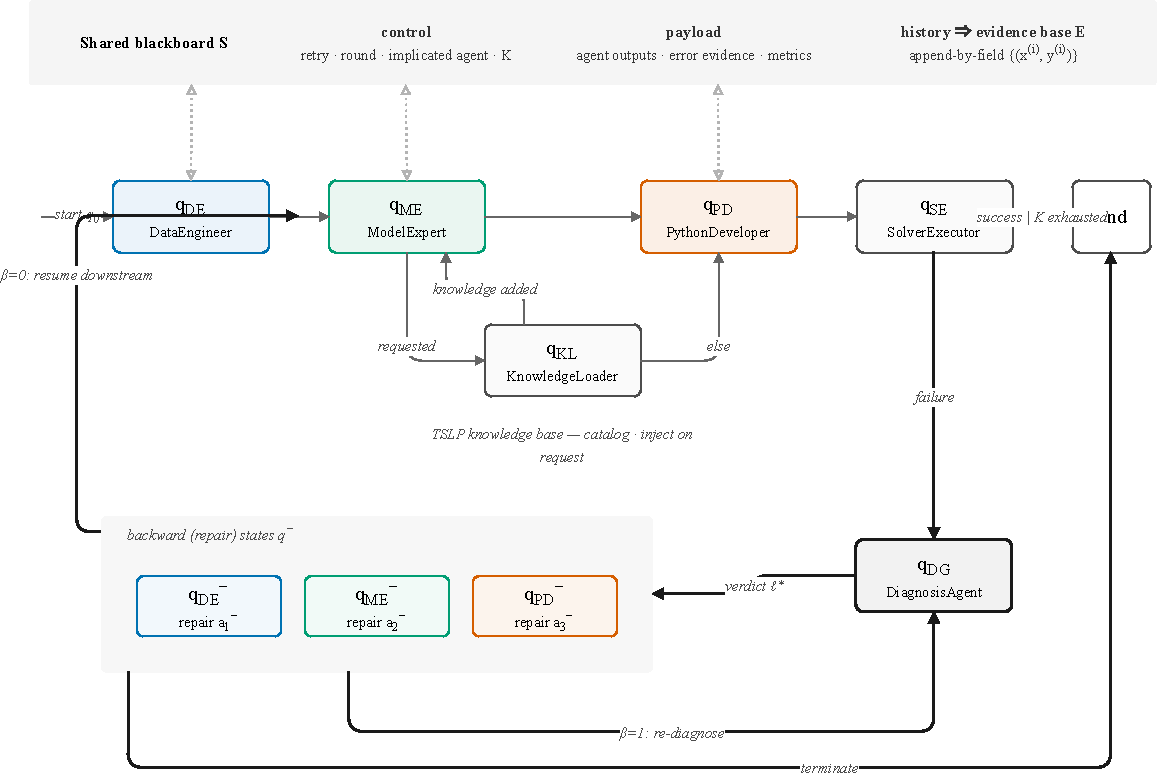
\includegraphics[width=0.95\linewidth]{fig_fsm.pdf}
\caption{The extended finite-state machine $M=(\Qcal,q_0,\Delta,\Scal,K)$.
Node colors mark the causally ordered correctable layers
data $\tri$ model $\tri$ code. $q_{\textsc{kl}}$ injects, on demand from a
catalogued TSLP knowledge base (two-stage structure; stage-1 sea and
stage-2 inland decisions $[\mathrm{D1}]/[\mathrm{D2}]$; network nodes;
demand scenarios $\Omega$; exogenous supply $\xi$; data layout), the
modules ModelExpert requests. Thin gray arrows: the forward chain. Bold
dark arrows: the
diagnosis--repair cycle --- the diagnosis verdict $\hat{\ell}^{\star}$
selects the backward state, and the return transition $\delta^{-}$ routes on
the executed Stackelberg verdict (Section~\ref{sec:stackelberg}): resume
downstream of the repaired agent ($\beta{=}0$), re-enter diagnosis
($\beta{=}1$), or terminate. Dotted stubs: every state reads from and
writes to the shared blackboard $\Scal$ only, whose append-by-field history
constitutes the evidence base $\Ecal$ of the inspection game.}
\label{fig:fsm}
\end{figure}

\paragraph{Transitions are pure functions of the blackboard.} The transition
map $\Delta$ is realized by five routing functions, each a pure map
$\Scal\to\Qcal$:
\begin{itemize}
    \item $\delta_{\textsc{me}}$: after ModelExpert, branch to
    \textsc{KnowledgeLoader} iff it requests not-yet-loaded modules, else to
    PythonDeveloper;
    \item $\delta_{\textsc{kl}}$: after KnowledgeLoader, return to ModelExpert
    iff new knowledge was added, else proceed to PythonDeveloper;
    \item $\delta_{\textsc{se}}$: after SolverExecutor, terminate on success
    or budget exhaustion, otherwise route to DiagnosisAgent;
    \item $\delta_{\textsc{dg}}$: after DiagnosisAgent, route to the backward
    state of the implicated agent (the diagnosis verdict);
    \item $\delta^{-}$: after a backward step, either resume the pipeline
    downstream from the repaired agent, re-enter diagnosis, or terminate ---
    depending on whether the repair was accepted and which agent was repaired.
\end{itemize}
The retry budget $K$ (\texttt{max\_retries}) bounds the number of
diagnosis--repair cycles, i.e., it is the FSM's transition budget over the
diagnostic sub-graph.

\paragraph{Domain knowledge is progressive scaffolding, not the contribution.}
ModelExpert does not receive a dump of every domain file, nor a RAG retriever.
It first sees a \emph{catalog} (module name + short description); it may then
request modules by name; \textsc{KnowledgeLoader} injects only those full
texts and returns control for refinement. This on-demand path is required for
correct TSLP modeling but is orthogonal to the Stackelberg inspection game:
both features plug into the same FSM without owning each other's logic.

\paragraph{The FSM is the stage-game apparatus, not scaffolding.} The state
machine is the structural substrate of the contribution because it is the
object on which the repair game is defined. Its states are stage-game states,
and --- once the repair game is in play --- the transitions
$\delta_{\textsc{dg}}$ and $\delta^{-}$ become functions of the players'
strategy profile (the inspector's committed inspection policy and the
inspectee's verified response; Section~\ref{sec:stackelberg}) rather than of a
fixed heuristic. Treating $M$
as the stage-game apparatus is what lets the commitment order carry
\emph{causal} meaning and what supports the proposition in
Section~\ref{sec:stackelberg}; without this formalization, the FSM would be
indistinguishable from generic graph orchestration.

%------------------------------------------------------------------------------
\subsection{Inter-agent communication via a shared blackboard}
\label{sec:comm}

Agents never exchange messages pairwise. All communication is mediated by a
single typed blackboard $\Scal$ (realized as the \texttt{AgentState} schema):
every node reads its inputs from $\Scal$ and writes its outputs back to
$\Scal$, and the transition functions $\Delta$ route solely on $\Scal$'s
contents. This \emph{shared-state, no-direct-links} design has three
consequences.

\paragraph{Control and payload on one schema, separated by reader.} $\Scal$
carries both \emph{control state} and \emph{data payload}. Control fields ---
retry count, the currently implicated agent, a resolved flag, the diagnosis
mode, the round counter, the retry budget --- drive $\Delta$ and are the only
fields a routing function inspects. Data fields --- each agent's output, the
assembled error evidence, execution metrics, the loaded knowledge modules, and
the ground-truth objective --- carry the pipeline's content and are read by the
agent that fires next. Colocating these concerns on one schema while
separating their readers is what makes the FSM's transitions both data-aware
and cheap to reason about.

\paragraph{A consistent, fixed data view.} A deterministic preprocessor runs
once, before any LLM agent fires, and writes a canonical view of the raw
instance into $\Scal$. Every downstream agent therefore reasons over an
identical data basis, eliminating a class of data-parsing races that would
otherwise masquerade as modeling or coding errors and confuse the diagnosis
mechanism.

\paragraph{Append-by-field history.} Communication is append-by-field rather
than overwrite: a backward step writes a corrected output together with a
resolved flag without erasing the prior forward outputs. The diagnosis
mechanism can therefore inspect the full input--output history
$\{(x^{(i)},y^{(i)})\}$ when attributing a failure. This history is the
evidence base $\Ecal$ on which the Stackelberg game of
Section~\ref{sec:stackelberg} is defined, and its completeness is what makes
blame attributable rather than heuristic.

%------------------------------------------------------------------------------
\subsection{The Stackelberg diagnosis--repair game as an inspection game}
\label{sec:stackelberg}

We cast the diagnosis--repair stage as a
Stackelberg game on the FSM multi-agent pipeline. The DiagnosisAgent moves
first and commits --- observably --- to an inspection policy; the accused
correctable agents then best-respond. Leader commitment plus follower
response matches the pipeline's control structure: the orchestrator already
routes through diagnosis before any repair is applied, so the natural
extensive form is sequential rather than simultaneous classification.

\subsubsection{Causal layering of defects and the deflection incentive}
\label{sec:layered}

Let the correctable core of the pipeline be the chain
$a_1\tri a_2\tri a_3$ (DataEngineer $\tri$ ModelExpert $\tri$ PythonDeveloper),
i.e.\ \emph{data $\tri$ model $\tri$ code}, where $\tri$ denotes ``is a causal
prerequisite of.'' We assume \emph{strict causal layering of defects}: a defect
introduced at layer $\ell\in\{1,2,3\}$ may manifest at any layer $j\ge \ell$,
but a defect at layer $\ell$ cannot be the root cause of a symptom that
requires only layers $<\ell$ to be well-formed. Consequently, the observation
of a downstream failure (e.g.\ an infeasible solve, a wrong objective, or a
traceback into solver-facing code) is consistent with several root-cause
layers, and localizing the true root cause $\ell^{\star}$ from the failure
evidence $\Ecal$ alone is fundamentally ambiguous: $\Ecal$ records the
\emph{symptom locus} (often $a_3$), not a certified identity of
$\ell^{\star}$. In particular, one cannot read the root-cause layer off the
\texttt{SolverExecutor}'s failure surface alone: a Python traceback or crash
locus typically marks where the pipeline \emph{broke}, most often in
generated code, rather than where the defect was \emph{introduced}. The
failure surface therefore motivates an \emph{inspection} protocol rather than
a one-shot classification of the traceback locus.
Figure~\ref{fig:layering} sketches this structure.

\begin{figure}[pos=htbp]
\centering
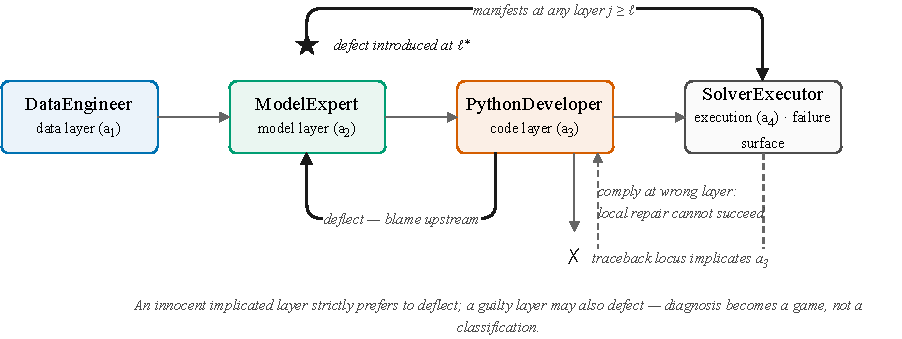
\includegraphics[width=0.95\linewidth]{fig2_causal_layering.pdf}
\caption{Causal layering of defects and the deflection incentive
(Section~\ref{sec:layered}). A defect introduced at layer $\ell^{\star}$
(star) propagates strictly downstream and may manifest at any layer
$j\ge\ell$; the SolverExecutor failure surface records the symptom locus
(often generated code), not the certified root cause. Reading the traceback
locus therefore implicates $a_3$ heuristically (dashed arrow). An
implicated-but-innocent layer strictly prefers to \emph{deflect} (bold
arrow): a local repair cannot succeed and only consumes tokens, so
complying at the wrong layer fails re-solve ($\times$). A guilty layer may
likewise defect to dodge the repair cost --- this misalignment is what turns
diagnosis into an inspection game rather than a classification.}
\label{fig:layering}
\end{figure}

Causal layering of defects does not merely make attribution ambiguous; it
gives the accused agents \emph{misaligned private incentives}, which is what
turns diagnosis into a game rather than a classification. Consider an agent
at layer $\ell$ that a failure has implicated. Two facts hold simultaneously:
(i) repair is costly --- a backward step re-generates the agent's output,
consumes tokens, and risks injecting a fresh defect; and (ii) if
$\ell\neq\ell^{\star}$ (the layer is innocent, merely downstream of the true
cause), then \emph{no} local repair at $\ell$ can make the solve pass,
because by strict causal layering of defects the true defect lies upstream.
An innocent implicated agent therefore strictly prefers to \emph{deflect}
--- to rebut the accusation and point blame upstream --- rather than to
accept a repair that wastes effort and cannot succeed. Symmetrically, even a
guilty layer, if it could avoid the repair cost by deflecting, would be
tempted to do so. The accused agents are thus not neutral truth-seekers whose
objective coincides with the diagnostician's; they are self-interested
inspectees. Resolving this requires an inspector that \emph{commits} to
verification, which is what Section~\ref{sec:stage_game} constructs.

This incentive structure is exactly that of an inspectee facing an inspector.
We accordingly specialize the stage game to a Stackelberg
\emph{inspection game}~\citep{avenhaus2002inspection,maschler1966inspection},
a canonical class of leader--follower games in which an inspector commits to a
monitoring policy and an inspectee best-responds. The diagnosis agent is the
inspector (leader); the accused correctable agents are inspectees (followers);
and the inspector's first-mover \emph{commitment} to a causal-order,
executed-refutation policy is what induces truthful attribution as the
inspectees' best response. Table~\ref{tab:game_mapping} maps the
inspection-game elements to the pipeline and contrasts them with
non-committed, single-judge protocols.

\begin{table}[pos=htbp]
\centering
\small
\caption{Mapping of Stackelberg inspection-game elements to the
diagnosis--repair stage. Right column: what non-committed / single-judge
protocols provide instead.}
\label{tab:game_mapping}
\begin{tabularx}{\linewidth}{>{\raggedright\arraybackslash}X >{\raggedright\arraybackslash}X >{\raggedright\arraybackslash}X}
\toprule
Inspection-game element & Concretization in our mechanism & Non-committed / single-judge protocols \\
\midrule
Inspector / leader (moves first, commits) & DiagnosisAgent commits an inspection policy $\sigma$: probe order + executed refutation & One LLM call picks a suspect \\
Inspectees / followers (best-respond) & Accused agents $a_1,a_2,a_3$: comply-and-repair or deflect-upstream & Accused agent self-checks in isolation \\
Committed policy $\sigma$ & Causal-order probing + verify by real re-solve (no cheap talk) & Fixed heuristic prior + single confidence \\
Conflict of interest & Innocent layer deflects to avoid wasted repair / wrongful blame & (assumed absent) \\
Inspector payoff & Correct root-cause localization at fewest rounds/tokens & (undefined) \\
Inspectee payoff & Avoid wrongful blame and wasted repair; fix only if truly at fault & A confidence score \\
Induced outcome & Guilty layer complies; innocent deflection is verified & Confidence-routed re-accusation \\
Stage-game apparatus & The LangGraph FSM (states = stage-game states) & (treated as plumbing) \\
\bottomrule
\end{tabularx}
\end{table}

\subsubsection{Game formulation}
\label{sec:stage_game}

A diagnosis--repair stage game $G$ is instantiated whenever $\Delta$ routes
from $q_{\textsc{se}}$ to $q_{\textsc{dg}}$ (the solver has failed and the
budget is not exhausted). The game is played on the current blackboard
$S_t\in\Scal$ and has the following structure.

\paragraph{Players.} An \emph{inspector} $I$ (the leader) and a set of
\emph{inspectees} (the followers). The inspector is the DiagnosisAgent $a_5$,
operating as an independent examiner. The inspectees are the correctable
agents $a_1,a_2,a_3$; in a given probe the active inspectee is the agent
$a_{\hat{\ell}}$ at the currently probed layer $\hat{\ell}$.

\paragraph{Timing.} Play is Stackelberg: the inspector first commits to an
observable inspection policy; the active inspectee then responds; the
inspector finally settles the response by verification. The probing order
$\omega$ follows the causal order $a_1\tri a_2\tri a_3$: the inspector probes
the seeded suspect layer first and, when a layer is cleared, descends to the
next causal layer. Aligning commitment order with causal order makes the
first move causally meaningful (an upstream probe is settled by re-solve
before the inspector descends) rather than a coin flip among
observationally equivalent layers.

\paragraph{Strategies.} The inspector's strategy is an \emph{inspection
policy} $\sigma=(\omega,\,\nu)$ fixed \emph{before} any inspectee responds:
(i)~a probing order $\omega$ over the layers, and (ii)~a verification rule
$\nu$ that resolves every response by \emph{executed refutation} rather than
by accepting the inspectee's word. When probed at layer $\ell$, the inspectee
chooses
$r\in\{\textsc{comply},\textsc{deflect}\}$. To \textsc{comply} is to accept
responsibility and emit a concrete repair $h\in\mathcal{H}_{\ell}$; to
\textsc{deflect} is to rebut the accusation and assert that the root cause
lies upstream. Given evidence $\Ecal$ from the blackboard --- stack trace,
solver log, implicated code, model definition, data structures, and pipeline
input--output pairs $\{(x^{(i)},y^{(i)})\}$ --- the active inspectee emits
\begin{equation}\label{eq:inspectee}
(r,\,h)\;\gets\; a_{\hat{\ell}}^{-}\!\bigl(x^{(\hat{\ell})},\,y^{(\hat{\ell})},\,\Ecal\bigr),
\qquad r\in\{\textsc{comply},\textsc{deflect}\},
\end{equation}
where, if $r=\textsc{comply}$, $h$ carries a justified repair, and if
$r=\textsc{deflect}$, $h$ carries an upstream rebuttal.

\paragraph{Verification.}
\label{sec:leader_follower}
Under its committed rule $\nu$, the inspector does not take the response on
trust. It selects and \emph{executes} the cheapest decisive test,
\begin{equation}\label{eq:follower}
\tau^{\star} \;\gets\; \arg\min_{\tau\in\mathcal{T}(r,h)}\,
      \mathrm{cost}(\tau)\quad\text{s.t.\ $\tau$ is decisive,}
\end{equation}
--- a re-solve after applying $h$ when $r=\textsc{comply}$, or a targeted
re-solve isolating the named upstream layer when $r=\textsc{deflect}$ --- and
issues a verdict
\begin{equation}\label{eq:verdict}
v \;=\; \bigl(\,\beta,\;\hat{\ell}^{\star}\,\bigr)
\;=\; I\!\bigl(r,\,h,\,\tau^{\star},\,S_t\bigr),
\end{equation}
where $\beta\in\{0,1\}$ records whether the probed layer is \emph{cleared}
($\beta{=}1$: a compliance whose re-solve still fails, or a deflection the
inspector upholds) or \emph{confirmed} ($\beta{=}0$: a compliance whose
re-solve passes the strict-success rule), and $\hat{\ell}^{\star}$ is the
updated root-cause estimate. Executing the test supplies a grounded signal:
neither a false confession nor a dishonest deflection survives. The FSM
transition $\delta^{-}$ routes on this verdict: if $\beta=0$, the repair in
$h$ is committed and $\Delta$ resumes downstream of $a_{\hat{\ell}}$; if
$\beta=1$, $\Delta$ re-enters diagnosis and the inspector probes the next
causal layer, until confirmation or budget exhaustion ($K$).

\paragraph{Payoffs.}
\label{sec:payoff}
Because LLMs admit no stable, observable utility function, we do \emph{not}
claim that an LLM ``feels'' a payoff. Instead we define numeric payoffs that
the orchestrator optimizes and treat each LLM call as a \emph{black-box
best-responder}, analyzing the resulting trajectory. The inspector's payoff
rewards correct localization at low cost,
\begin{equation}\label{eq:ui}
u_{I}(\sigma) = \mathbf{1}\!\bigl[\,\hat{\ell}^{\star}=\ell^{\star}\bigr]
                 \;-\;\lambda_{I}\,\mathrm{cost}(\sigma),
\end{equation}
while the inspectee at layer $\ell$, responding $r$, has the misaligned payoff
\begin{equation}\label{eq:ue}
u_{\ell}(r;\sigma) =
   b\cdot\mathbf{1}\!\bigl[\,r{=}\textsc{comply}\wedge\text{re-solve passes}\bigr]
   \;-\;c_{\mathrm{rep}}\,\mathbf{1}\!\bigl[\,r{=}\textsc{comply}\bigr]
   \;-\;c_{\mathrm{blame}}\,\mathbf{1}\!\bigl[\,\text{held responsible}\wedge \ell\neq\ell^{\star}\bigr],
\end{equation}
where $b>0$ is the reward for actually resolving the failure,
$c_{\mathrm{rep}}>0$ the cost/risk of a repair, $c_{\mathrm{blame}}>0$ the
penalty for carrying blame that does not fix the solve, $\mathrm{cost}(\cdot)$
is token/round cost, and $\lambda_{I}\ge 0$ trades accuracy against budget.
Eq.~\eqref{eq:ue} makes the conflict explicit: the inspectee is rewarded only
when it is \emph{both} at fault \emph{and} repairs, and is otherwise penalized
for complying, so its interests diverge from the inspector's whenever
$\ell\neq\ell^{\star}$. The ground-truth label $\ell^{\star}$ enters only the
\emph{evaluation} of payoffs, never any agent's prompt, so the game remains
well-defined at inference time; equilibria are properties of the
orchestrator-defined game, while each LLM is a sampled best-responder within
it.

\subsubsection{Induced truthful attribution}
\label{sec:deterrence}

The value of the inspector's first move is that its committed
executed-refutation rule $\nu$ reshapes the inspectee's best response ---
the classical inspection-game deterrence effect. Consider the two cases.
\emph{(i) Innocent inspectee} ($\ell\neq\ell^{\star}$): by strict causal
layering of defects a local repair cannot make the solve pass, so
\textsc{comply} yields $-c_{\mathrm{rep}}$ (no reward $b$, and it will still
be seen not to fix the solve), whereas a truthful \textsc{deflect} avoids the
repair cost and is upheld by the inspector's targeted re-solve. Deflection
strictly dominates --- and, crucially, only a \emph{truthful} deflection
survives $\nu$, since a dishonest one is refuted by re-solve.
\emph{(ii) Guilty inspectee} ($\ell=\ell^{\star}$): deflecting cannot succeed,
because every upstream probe the inspector runs under causal order passes
verification and the probe returns to $\ell^{\star}$ having only consumed
rounds; complying and repairing yields $b-c_{\mathrm{rep}}$. Whenever
$b>c_{\mathrm{rep}}$ (a resolved solve is worth more than the repair),
\textsc{comply} is the guilty layer's best response. Hence the committed
policy makes \emph{truthful attribution} --- the guilty complies, the
innocent deflects honestly --- the induced best-response profile. It is the
inspector's \emph{commitment}, not any assumed benevolence of the agents,
that aligns individually optimal responses with correct root-cause
localization. Without commitment, deflection is cheap talk and truthful
attribution is not incentive-compatible.

\emph{Information assumption.} The best-response analysis above assumes
the inspectee observes its own type ($\ell$ versus $\ell^{\star}$) before
responding. For LLM inspectees this is a behavioural idealization, not an
implementation fact: a comply/deflect output is one model reading the
blackboard evidence. The assumption is grounded exactly when the defect is
visible in the layer's own artifact --- a model-layer fault is inspectable
in the emitted formulation, so evidence-reading behaviour approximates the
informed best response --- and defeated by rank-invisible semantic data
faults. The measured comply/deflect profile (Section~\ref{sec:exp_diag})
is therefore read as evidence of how closely the implemented agents
approximate this intended equilibrium, not as a proof of it.

\subsubsection{Proposition}
\label{sec:proposition}

\begin{propbox}[title={Proposition 1 (Causal-order inspection lowers mis-attribution)}]
\emph{Premises.}
(A1)~Strict causal layering of defects (Section~\ref{sec:layered}): a defect
at layer $\ell$ cannot cause a symptom that requires only layers ${<}\ell$.
(A2)~No absorption: a repair emitted by an \emph{innocent} layer cannot pass
the executed re-solve.
(A3)~Repair sufficiency: a complying repair emitted by the \emph{guilty}
layer passes the executed re-solve.

\emph{Claim.} Under A1--A3 and an inspector committed to a causal-order,
executed-refutation policy, each probe is \emph{decisive} --- it confirms or
clears the probed layer --- and cleared layers are innocent, so the true
layer is never eliminated. Relative to a single-judge round, which produces
an unverified point hypothesis and therefore changes no layer's status,
every cleared probe strictly shrinks the viable root-cause set. Formally,
with $V_{\text{sim}}$ and $V_{\text{ins}}$ the sets of layers consistent
with the failure observation after one round of, respectively, single-judge
play (hence the full observationally-equivalent cone) and causal-order
inspection, $V_{\text{ins}}\subseteq V_{\text{sim}}$ with
$\ell^{\star}\in V_{\text{ins}}$, and the inclusion is strict whenever a
layer $\ell<\ell^{\star}$ is probed and cleared.
\end{propbox}

\emph{Proof.} An innocent probed layer cannot pass the re-solve by A2: its
compliance is refuted and its truthful deflection upheld, and either way it
is cleared --- so only innocent layers are ever cleared. For the guilty
layer, compliance is the best response (Section~\ref{sec:deterrence}) and
by A3 its repair passes, so it is confirmed and $\ell^{\star}$ is never
eliminated. A single-judge round executes no test, so no layer changes
status and $V_{\text{sim}}$ is the full observationally-equivalent cone;
inspection removes from it every cleared layer. $\square$

\emph{Status of the premises.} A1 is the structural assumption of
Section~\ref{sec:layered}; A2 and A3 are empirical regularities of the
implemented repair path, not axioms, and the measured campaign prices both.
Absorption (A2 failure) occurs on eight reverse-arm boards, where an
innocent code layer's free regeneration silently drops the upstream
constraint and passes the re-solve; repair insufficiency (A3 failure)
occurs on nine causal boards, where the guilty layer's complying repair is
overturned and the search moves past the true layer (both quantified in
the Exp-A mechanism findings, Section~\ref{sec:exp_ablation}).
The proposition delimits what commitment buys when the repair path
cooperates; the funnel measures how often it does.

%------------------------------------------------------------------------------
\subsection{The diagnosis--repair algorithm}
\label{sec:algorithm}

Algorithm~\ref{alg:fsm_stackelberg} unifies the architecture and the repair
game. The FSM drives the forward pass; on failure it enters the inspection
stage, where the inspector commits to a causal-order, executed-refutation
policy and probes layers in causal order --- each probe eliciting an
inspectee response and settling it by re-solve --- until a layer is confirmed
or the budget $K$ is spent. The transition map $\Delta$ is exactly the five
routing functions of Section~\ref{sec:architecture}, with the return edge out
of the backward state set by the executed verdict $v$.

\begin{algorithm}[htbp]
\caption{FSM-Stackelberg diagnosis--repair (inspection game)}\label{alg:fsm_stackelberg}
\begin{algorithmic}[1]
\Require Problem $\mathcal{P}$; agents $\{a_1,a_2,a_3,a_4\}$; inspector role $a_5$; FSM $M=(\Qcal,q_0,\Delta,\Scal,K)$; causal order $a_1\tri a_2\tri a_3$
\Ensure Result $Y\in\{\text{success},\text{failure}\}$
\State $S\gets\textsc{Preprocess}(\mathcal{P})$;\quad $k\gets 0$;\quad $Y\gets\bot$
\While{$Y=\bot$} \Comment{drive the FSM}
    \State \textit{\textbf{// Forward chain: $q_{\textsc{de}}\!\to\!q_{\textsc{me}}\!\to\!\{q_{\textsc{kl}}\}\!\to\!q_{\textsc{pd}}\!\to\!q_{\textsc{se}}$}}
    \For{$i=1$ \textbf{to} $4$}
        \State $y^{(i)}\gets a_i^{+}(S)$;\quad update $S$;\quad advance $\Delta$
    \EndFor
    \If{$y^{(4)}.\textsc{status}=\textsc{Optimal}$}
        \State $Y\gets\text{success}$
    \ElsIf{$k\ge K$}
        \State $Y\gets\text{failure}$
    \Else
        \State \textit{\textbf{// Inspection stage at $q_{\textsc{dg}}$: inspector commits $\sigma=$ (causal order, executed refutation)}}
        \State $\hat{\ell}\gets\textsc{Prior}(y^{(4)}.\textsc{status})$ \Comment{seed probe order}
        \Repeat
            \State $(r,h)\gets a_{\hat{\ell}}^{-}(S)$ \Comment{inspectee best-responds: comply-repair or deflect}
            \State $\tau^{\star}\gets\arg\min_{\tau\in\mathcal{T}(r,h)}\mathrm{cost}(\tau)$ s.t.\ decisive
            \State $(\beta,\hat{\ell}^{\star})\gets a_{5}\textsc{.verify}(r,h,\tau^{\star},S)$ \Comment{executed refutation (re-solve)}
            \State $k\gets k+1$
            \If{$\beta=0$} \Comment{layer confirmed} commit $\tilde{y}\in h$;\quad resume $\Delta$ downstream \EndIf
            \State $\hat{\ell}\gets\textsc{NextCausalLayer}(\hat{\ell})$ \Comment{layer cleared: descend causal order}
        \Until{$\beta=0\;\lor\;k\ge K$}
    \EndIf
\EndWhile
\State \Return $Y$
\end{algorithmic}
\end{algorithm}

\paragraph{Relation to the baseline.} The forward chain, the blackboard, and
the retry budget are inherited unchanged. The replacement is localized: the
single-judge diagnosis call and its confidence-routed return are substituted
by the committed inspection stage, and the return edge of $\delta^{-}$ is
driven by the executed verdict $\beta$ rather than by a confidence. This
locality is deliberate --- it isolates the contribution (the inspection game)
from the scaffolding (the FSM) and makes the commitment-order ablation, which
randomizes the order in which layers are probed, the decisive experiment: if a
permuted order performs as well as causal order, the thesis is falsified.

%==============================================================================
\section{Experiments}
\label{sec:experiments}

The campaign tests whether a committed inspection policy improves
\emph{verifiable} root-cause attribution under layered faults---and whether
it can match a strong single-judge LLM on naming accuracy---rather than
whether any protocol can eventually repair a failed solve.
\paragraph{Claim and mechanism under test.}
We do not claim that Stackelberg inspection is uniquely able to name
$\ell^{\star}$ from a stack trace: at failure time every method sees the same
blackboard, so a capable single-judge LLM may match first-shot accuracy.
The intended footing is the conjunction of (i)~accuracy that is at least
competitive with single-judge diagnosis, (ii)~\emph{verifiable} attribution
via commitment plus executed refutation, and (iii)~cost/audit properties
under the same budget $K$. Achieving (i) requires an
\emph{evidence-informed} commitment: the leader forms a \emph{layer ranking}
from the stack and agent histories (ranks or votes---\emph{not} LLM-reported
probabilities, which are poorly calibrated), commits $\omega$, then probes
with executed refutation. Status-prior-only $\omega$ is treated as a
preliminary apparatus, not the final proposed policy.
\paragraph{Pre-registered expectations.}
Each experiment below states an \emph{expected conclusion} fixed before the
corresponding redesigned runs. The campaign is organized as three blocks:
commitment-order ablation, a unified baseline comparison (internal and
external protocols), and mechanism diagnostics. Tables marked
\emph{measured} report the evidence-informed redesign
(\texttt{omega\_source}=\texttt{evidence\_rank}, hybrid rank under the
force-zero plant); tables marked \emph{preliminary} are from the earlier
status-prior $\omega$ implementation and do not substitute for the redesign.
External Debate/Reflexion ran later under the same engine and snapshot
protocol (measured below); Exp-C remains unrun at the time of writing.

\subsection{Setup}
\label{sec:exp_setup}

\paragraph{Data.}
All methods use the demand-uncertainty TSLP ECR model of
Section~\ref{sec:ecr_model} on the exported dataset
\texttt{prob\_\allowbreak tslp\_\allowbreak ecr\_\allowbreak demand}. We start from the smoke instance
\texttt{smoke\_H4\_Omega5} and extend to a small family of
horizon/scenario configurations from the same generator. The forward
pipeline, blackboard schema, strict-success rule
(Table~\ref{tab:outcome_taxonomy}), and sandbox solver path are shared. An
end-to-end smoke run on \texttt{smoke\_H4\_Omega5} with progressive knowledge
injection terminated in \emph{Practical Optimal}
($\hat{z}\approx z^{\star}\approx 1.390\times 10^{6}$, relative gap below the
$10^{-3}$ threshold): the solver's \textsc{Optimal} status was therefore
\emph{not} a Spurious Optimal under the taxonomy above.

\paragraph{Model and budget $K$.}
Provider and model are held fixed within each comparison block and reported
explicitly. Every method receives the same retry budget $K$
(\texttt{max\_retries}); the single declared exception is the Reflexion
budget-tilted challenger sweep at $K{=}5$
(Section~\ref{sec:exp_baselines}).

\paragraph{Injection protocol.}
Ground-truth root causes $a^{\star}\in\{a_1,a_2,a_3\}$ are obtained by
controlled injection: a defect is planted at one of the three layers
(DataEngineer, ModelExpert, or PythonDeveloper) so that the surface
symptom often appears downstream (e.g., a traceback or crash locus in
generated code, or a feasible-but-wrong optimum). The measured grids use
three plants, one per layer: \texttt{me\_force\_zero\_sea}
($a^{\star}$=ModelExpert), \texttt{pd\_comment\_out\_balance}
($a^{\star}$=PythonDeveloper; balance constraints commented out of
generated code), and \texttt{de\_swap\_demand\_supply\_source}
($a^{\star}$=DataEngineer; a contract-valid semantic swap of demand and
supply catalog sources). This matches the motivation in
Section~\ref{sec:stackelberg} that failure evidence records a symptom locus,
not a certified identity of $\ell^{\star}$. The label $a^{\star}$ is used only
for evaluation, never in agent prompts.

\paragraph{Fairness.}
At failure time every method reads the same blackboard (solver status, stack
trace, agent input--output history). Repair uses the same agent
\texttt{backward\_step} maps and the same re-solve verification path;
methods differ only in how they select or order the implicated layer. No
method receives privileged tools beyond its diagnosis policy. In snapshot
mode (below) the same-blackboard promise is exact by construction: the
failure state is frozen once per seed and all arms resume it verbatim.

\subsection{Methods compared}
\label{sec:exp_methods}

\begin{itemize}
    \item \textbf{(A) Proposed / ablation family.}
    \texttt{diagnosis\_mode}=\texttt{stackelberg} with committed policy
    $\sigma=(\omega,\nu)$ and $\nu$ fixed as executed refutation. The leader
    forms an evidence-informed layer ranking (no confidence weights), then
    commits a probing order $\omega\in\{\texttt{causal},\texttt{reverse},
    \texttt{random}\}$ obtained by aligning that ranking with
    (or permuting against) the data$\tri$model$\tri$code skeleton.
    \item \textbf{(B) Internal baselines} (Exp-B, same table as C).
    (i)~\texttt{adversarial}: single-judge LLM accusation plus accused-agent
    self-check; (ii)~\texttt{sequential}: fixed reverse-order backward chain
    without an inspection commitment.
    \item \textbf{(C) External verification baselines} (Exp-B).
    (i)~\emph{Debate}~\citep{du2023improving}: multiple diagnosis personas
    argue for a fixed number of rounds; terminal positions are aggregated by
    majority vote (no LLM-reported confidence weights; ties broken by the
    status prior), then the accused layer enters the shared repair/re-solve
    path. (ii)~\emph{Reflexion}~\citep{shinn2023reflexion}: single-judge-style
    accusation augmented with verbal reflections after failed
    diagnose--repair attempts, conditioned upon in later diagnosis rounds,
    again sharing the same repair/re-solve machinery.
    Internal and external protocols answer one baseline question and are
    reported together in Section~\ref{sec:exp_baselines}; execution may stage
    (B) before (C) for cost control.
\end{itemize}

\subsection{Metrics}
\label{sec:exp_metrics}

The primary metric is \emph{verified} root-cause attribution accuracy
$\mathbf{1}\{\hat{a}=a^{\star}\}$ where $\hat{a}$ is the layer supported by
executed refutation (not merely last-comply credit), optionally stratified by
injected origin and solver-status surface. For commitment-order contrasts we
also report the first-probe hit $\mathbf{1}\{\omega_1=a^{\star}\}$ --- a
\emph{commitment-side} quantity: under the committed policy the engine
routes every probe to the first not-yet-cleared layer of $\omega$, so the
executed first probe coincides with $\omega_1$ by construction and the
metric reads out whether the committed order --- rank-aligned (causal),
reversed, or shuffled (random) --- targeted the true layer. Its
outcome-side complement is \emph{first-probe confirmation}: the probed
guilty layer complies and its repair passes the executed re-solve at the
first probe (equivalently, verified attribution at $K{=}1$). Confirmation
requires alignment \emph{and} repairability, and the gap between the two
metrics locates the repair path's failure modes. Secondary
metrics are SSR@$K$, probe rounds, and loop tokens (total minus the
frozen forward prefix, Section~\ref{sec:exp_reporting}). SSR counts only
\emph{Practical Optimal} outcomes in Table~\ref{tab:outcome_taxonomy}; a bare
\textsc{Optimal} that fails the $z^{\star}$ gap test
(\emph{Spurious Optimal}) does not contribute. For
Exp.~\ref{sec:exp_diag} we additionally record deflect rates, the fraction of
compliances and deflections overturned by executed refutation, and
analysis-mode episode payoffs $(u_L,u_F)$ from Section~\ref{sec:payoff}.
Highest SSR alone is not a sufficient claim: under strong models many
protocols may eventually repair; the scientific contrast is verifiable
attribution under commitment at competitive naming accuracy.

\subsection{Result interpretation and provenance}
\label{sec:exp_reporting}

\paragraph{Reading results against expectations.}
Pre-registered expectations are the reading grid for every table that
follows: an outcome \emph{supports}, \emph{does not support}, or
\emph{falsifies} the registered expectation, and an unsupported
expectation revises the design before further experimental spend rather
than accumulating post-hoc explanations. The campaign has already exercised
this rule once. The status-prior implementation failed its attribution
expectations outright---last-comply attribution was $0/5$ for every method
in the baseline comparison (Table~\ref{tab:exp_baselines_prelim}), and no
order exceeded $1/5$ in the ablation
(Table~\ref{tab:exp_ablation_prelim})---and the recorded response was a
redesign of the commitment apparatus (evidence-informed ranking plus
verified attribution accounting), not a re-labelling of the old runs; the
status-prior tables are retained below only as preliminary context. The
grid was run under sequential disclosure: an $n{=}3$ feasibility pass, an
interim inspection at $n{=}5$, an expanded $n{=}20$ campaign, and a further
densification to $n{=}30$, all with unchanged expectations; freeze-phase
attempts that never produce a failure
blackboard (data-contract rejections by the deterministic validator, or
plants not expressed in the generated model) are reported as forward
variance and replaced with fresh seeds, never silently dropped.
Confirmatory claims below are restricted to the clauses the expanded grid
can power (first-probe); verified-attribution contrasts that remain
non-significant are stated as such. SSR is never interpreted in isolation
from attribution (Section~\ref{sec:exp_metrics}).

\paragraph{Provenance and implementation versions.}
Every measured cell is produced by a single frozen implementation. Each run
writes a machine-readable manifest (configuration, provider and model,
terminal metrics) and a per-node event log (tokens, durations,
comply--deflect responses); tables aggregate these records, and the
manifests and event logs---not any intermediate summary file---are the
authority for every number reported. Implementation versions are declared
rather than silently mixed. The measured tables below were produced under
the hardened data layer (deterministic catalog and validator constraining
the data-access guide in forward and backward passes), re-established
after a no-plant end-to-end gate terminated in \emph{Practical Optimal}
(measured relative gap $0.0\%$, far below the $10^{-3}$ threshold), on
provider DeepSeek /
\texttt{deepseek-flash} (thinking disabled, temperature $0$), and in
\emph{snapshot mode}: the failure blackboard is frozen once per seed at
the solver$\to$diagnosis boundary and every arm resumes the identical
board, so order arms are paired on the same failure state by construction;
token costs are \emph{loop tokens} (total minus the frozen forward
prefix). Earlier DashScope $n{=}3$ cells predate this campaign and are
neither pooled nor compared numerically; each table carries the campaign,
and hence the implementation freeze, it was produced under. One
classification parameter was tightened during analysis and is disclosed
here rather than silently applied: the strict-success gap threshold moved
from $10^{-2}$ to $10^{-3}$. The choice is data-driven rather than
arbitrary: across the $316$ measured runs with a computable gap the
distribution is sharply bimodal---exactly $0.0000\%$ for $184$ runs and at
least $1.01\%$ for $129$, with only three cells in between ($0.03\%$,
$0.53\%$, $0.99\%$)---and the instances are LPs whose deterministic
equivalents two exact solvers agree on to $\sim10^{-9}$ relative, so the
in-between cells are real model deviations rather than solver noise. All
tables below were recomputed offline from the run manifests---the
authority for every number---under the tightened rule; exactly two cells
reclassify from Practical Optimal to Spurious Optimal (one Debate
external cell at $0.53\%$, one random-order ablation cell at $0.99\%$),
both in arms competing with causal Stackelberg, and no directional
conclusion changes.

\subsection{Exp-A: Commitment-order ablation}
\label{sec:exp_ablation}
\label{sec:exp_i}

\paragraph{Question.}
Does the inspector's committed probing order carry information under layered
faults? Equivalently: holding $\nu$ and $K$ fixed, is causal-order commitment
better than reverse or random commitment on first-probe hit and verified
attribution?

\paragraph{Design.}
All cells use \texttt{diagnosis\_mode}=\texttt{stackelberg} with evidence-informed
ranking at commit time. We vary only
$\omega\in\{\texttt{causal},\texttt{reverse},\texttt{random}\}$ on the
injection grid of Section~\ref{sec:exp_setup}. Causal $\omega$ rotates the
data$\tri$model$\tri$code skeleton so that the top-ranked layer is probed
first; reverse and random break that alignment (and, per the redesign spec,
do not reuse the rank tip), isolating order from naming skill.

\paragraph{Expected conclusion.}
Causal $\omega$ yields strictly higher first-probe hit and verified
attribution than reverse, and at least weakly higher than random, at
comparable token cost. If causal $\approx$ random/reverse,
Proposition~1 carries no empirical bite and the ranking/alignment design
is revised before baselines.

\paragraph{Measured results (evidence-informed; snapshot mode; $n{=}30$/order).}
Table~\ref{tab:exp_ablation} reports the expanded ablation on
\texttt{smoke\_H4\_Omega5} with plant \texttt{me\_force\_zero\_sea},
$K{=}3$, provider DeepSeek / \texttt{deepseek-flash}, and
\texttt{rank\_method}=\texttt{hybrid} (the force-zero smell tips
\texttt{model\_expert} without inventing a second diagnosis mechanism).
Causal commitment attains first-probe $30/30$ versus $15/30$ under random
and $0/30$ under reverse (paired exact McNemar: $30{:}0$ discordant
pairs, $p=1.9\times10^{-9}$, and $15{:}0$, $p=6.1\times10^{-5}$): the
registered first-probe clause is strongly supported. Verified
attribution is $14/30$ causal, $13/30$ random, $7/30$
reverse; the causal-versus-reverse contrast is significant
($8{:}1$ discordant pairs, $p=0.039$), and causal versus random remains a
near-tie ($5{:}4$, $p=1.0$)---the weak clause is met as a tie. Two
mechanism findings qualify these counts. First, first-probe naming is
commitment-side by construction
(Section~\ref{sec:exp_metrics}): the executed first probe equals
$\omega_1$ on every board, verified event-by-event against the logs, so
the hit counts measure which orders targeted the guilty layer --- the
hybrid rank names the model layer on all $30$ boards, and exactly the
$15$ random shuffles that placed it first hit. The outcome-side quantity
is the confirmation funnel: of causal's $30$ aligned first probes, $14$
confirm (guilty-layer comply, re-solve passes); the remaining $16$ split
into $9$ whose model-layer repair is overturned by the re-solve and the
run ends in terminal failure (final relative gaps $1.7$--$55.8\%$), and
$7$ where the model repair is correct but the downstream code
regeneration injects a fresh defect, the next probe credits the code
layer, and the run terminates \emph{Practical Optimal} without verified
attribution --- the whole of causal's SSR margin ($21{=}14{+}7$). Random
mirrors the funnel on its aligned half ($9$ of $15$ confirm; the other
$6$ are overturned terminal failures), and reverse exposes the converse
hazard: on $8$ boards an \emph{unaligned} first probe absorbs the
model-layer fault outright --- the regenerated code silently drops the
injected constraint, the re-solve passes, and the credit settles on the
code layer; these eight boards are more than half of reverse's SSR
($8$ of $15$) and none is a verified attribution. Second, $4$ of the
random arm's $13$ verified attributions start from \emph{unaligned}
shuffles and still reach the guilty layer by executed refutation within
$K$: alignment raises the chance of early verified attribution, but
multi-round search under executed refutation is a genuine second route.
Token costs are of the same order across orders (causal marginally
lowest). Figure~\ref{fig:expa} summarizes the ablation and the alignment
audit.

\begin{figure}[pos=htbp]
\centering
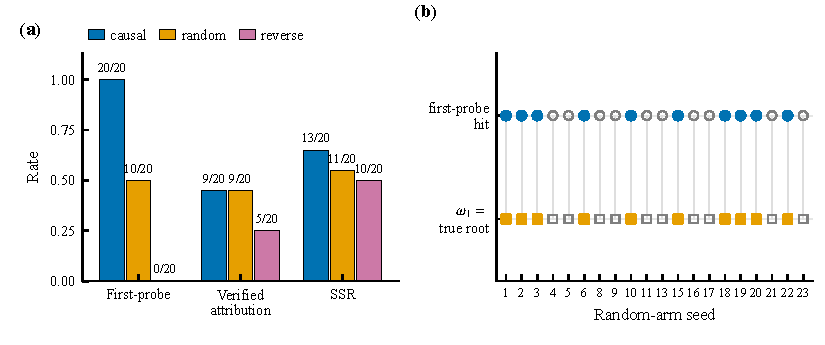
\includegraphics[width=0.85\linewidth]{fig5_exp_a_ablation.pdf}
\caption{Exp-A commitment-order ablation and alignment audit (measured;
snapshot mode; $n{=}30$/order; plant \texttt{me\_force\_zero\_sea}).
(a) First-probe hit, verified attribution, and SSR@$K$ by probe order.
(b) Seed-level audit of the random arm: the executed first probe equals
the committed $\omega_1$ on every board (probing is bound to the
commitment), so naming hits are exactly the shuffles that place the
guilty layer first ($15/15$) --- the random arm's
naming performance is carried entirely by accidental alignment with the
ranking. Freeze attempts that produced no failure blackboard (seeds 7,
12, 14, 24, 25, 27, 28; data-contract rejections) are outside the
campaign's $n{=}30$.}
\label{fig:expa}
\end{figure}

\begin{table}[t]
\centering
\caption{Exp-A commitment-order ablation --- \textbf{measured}
(evidence-informed; snapshot mode; $n{=}30$/order; $K{=}3$; hybrid rank;
DeepSeek \texttt{deepseek-flash}; plant \texttt{me\_force\_zero\_sea};
loop-token accounting). Primary: first-probe hit and verified
attribution.}
\label{tab:exp_ablation}
\label{tab:exp_i}
\begin{tabular}{@{}l c c c c@{}}
\toprule
$\omega$ & First-probe hit & Verified attr.\ & SSR@$K$ & Mean loop tokens \\
\midrule
causal  & $30/30$ (1.00) & $14/30$ (0.47) & $21/30$ & $0.64{\times}10^{5}$ \\
random  & $15/30$ (0.50) & $13/30$ (0.43) & $17/30$ & $0.67{\times}10^{5}$ \\
reverse & $0/30$ (0.00) & $7/30$ (0.23) & $15/30$ & $0.74{\times}10^{5}$ \\
\bottomrule
\end{tabular}
\end{table}

\paragraph{Multi-plant replication (Phase-4 grid; snapshot mode; $n{=}10$/order).}
Table~\ref{tab:exp_multiplant} replicates the ablation on the two
additional plants of Section~\ref{sec:exp_setup} under the identical
engine and protocol. The result is a \emph{conditional} replication that
revises the mechanism claim. On the code-layer plant
(\texttt{pd\_comment\_out\_balance}), causal attains $9/10$ first-probe,
significantly above random's $2/10$ ($7{:}0$ discordant pairs, $p=0.016$),
but reverse attains $10/10$: the reversed skeleton probes the code layer
first \emph{by construction}, so for a code-layer fault reverse is itself
the aligned order, and the registered ``strictly above reverse'' clause
cannot and does not hold ($0{:}1$). On the data-layer plant
(\texttt{de\_swap\_demand\_supply\_source}), the hybrid rank never names
the data layer (its smell rules cover force-zero and relaxed-DEP
surfaces, not contract-valid semantic source swaps): causal and reverse
both sit at $0/10$ first-probe and the clause is falsified there; the
only hits ($4/10$) are random shuffles that happened to align. Across all
three plants and all $40$ random-arm cells the executed first probe again
equals $\omega_1$ on every board, so the hits remain exactly the shuffles
that target $a^{\star}$ --- the empirical variable is which layer the
shuffle places first, not whether execution obeys the commitment.
Verified attribution shows no significant order
effect on either new plant (seed-level repairability and multi-round
refutation dominate at $K{=}3$). The grid also uncovered a
plant-specific forward-variance class: in $12$ of $22$ freeze attempts
for the data plant the swapped parameter never entered the generated
model and the run solved to the un-faulted optimum ($\hat z = z^{\star}$
to machine precision), leaving no failure blackboard; these attempts are
excluded and replaced with fresh seeds, and their $55\%$ rate is itself a
measured property of semantic data faults in LLM-generated pipelines.
The cross-plant reading is therefore not ``causal order wins'' but
\emph{alignment wins when the evidence ranking can see the fault layer}:
visible for the model-layer plant through the force-zero smell and for
the code-layer plant through the relaxed-DEP surface (and structurally
through reverse), invisible for the semantic data fault, where naming
fails for every fixed order and only chance alignment or multi-round
executed refutation recovers the root cause.
Figure~\ref{fig:visibility} condenses this conditional pattern.

\begin{figure}[pos=htbp]
\centering
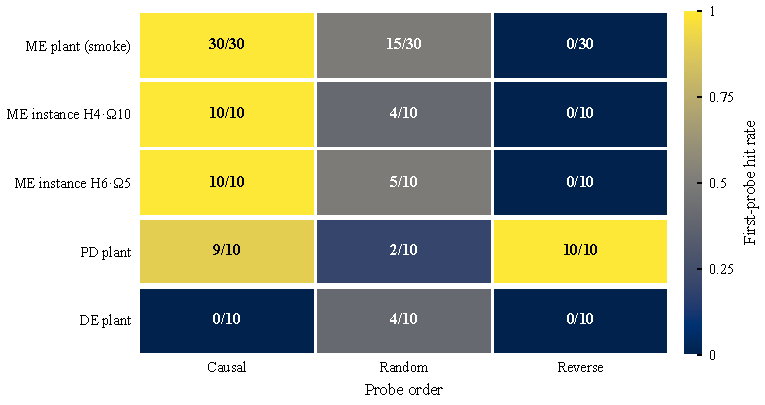
\includegraphics[width=0.72\linewidth]{fig6_visibility_matrix.pdf}
\caption{First-probe hit rate by plant/instance and probe order
(measured; snapshot mode; $K{=}3$; DeepSeek \texttt{deepseek-flash}). The
commitment-order effect is gated by fault visibility. Model-layer faults
(smoke plant and both instance replications) are visible to the causal
rank: causal $=1.0$, random $\approx 0.4$--$0.5$, reverse $=0$. The
code-layer fault is visible through the relaxed-DEP surface from
\emph{both} ordered endpoints (causal $9/10$, reverse $10/10$ by
construction) while random fails ($2/10$). The rank-invisible semantic
data fault defeats every fixed order (causal $=$ reverse $=0/10$); only
chance alignment (random $4/10$) or multi-round executed refutation
recovers it.}
\label{fig:visibility}
\end{figure}

\begin{table}[t]
\centering
\caption{Phase-4 multi-plant replication --- \textbf{measured} (snapshot
mode; $n{=}10$/order/plant; $K{=}3$; hybrid rank; DeepSeek
\texttt{deepseek-flash}; loop-token accounting). First-probe hit / verified
attr.\ / SSR@$K$ per order.}
\label{tab:exp_multiplant}
\begin{tabular}{@{}ll c c c c@{}}
\toprule
Plant ($a^{\star}$) & $\omega$ & First-probe & Verified attr.\ & SSR@$K$ & Loop tokens \\
\midrule
\texttt{pd\_comment} & causal  & $9/10$ & $5/10$ & $5/10$ & $0.85{\times}10^{5}$ \\
(\texttt{python})    & random  & $2/10$ & $2/10$ & $3/10$ & $0.68{\times}10^{5}$ \\
                     & reverse & $10/10$ & $5/10$ & $5/10$ & $0.51{\times}10^{5}$ \\
\midrule
\texttt{de\_swap}    & causal  & $0/10$ & $2/10$ & $6/10$ & $1.01{\times}10^{5}$ \\
(\texttt{data})      & random  & $4/10$ & $6/10$ & $8/10$ & $0.82{\times}10^{5}$ \\
                     & reverse & $0/10$ & $4/10$ & $6/10$ & $1.02{\times}10^{5}$ \\
\bottomrule
\end{tabular}
\end{table}

\paragraph{Instance-family replication (snapshot mode; $n{=}10$/order/instance).}
Table~\ref{tab:exp_instances} extends the model-layer plant to two
further instances exported from the same generator with a longer horizon,
a larger scenario set, and fresh base-data seeds (\texttt{fam\_H4\_Omega10}
and \texttt{fam\_H6\_Omega5}; each passed a no-plant end-to-end gate at
relative gap $0.0\%$ before faulting). The first-probe clause replicates
at full strength: causal attains $10/10$ on both instances and reverse
$0/10$; pooled over instances, causal versus reverse is $20{:}0$
discordant pairs ($p=2\times10^{-6}$) and causal versus random $11{:}0$
($p=0.001$), with the executed first probe again equal to $\omega_1$ on
every board. The clause the $n{=}20$ grid could not resolve is resolved on
the family and, after densification to $n{=}30$, on the main grid as well
(causal versus reverse $8{:}1$ discordant pairs, $p=0.039$):
verified attribution is strictly higher under causal ($0.70$ and $0.50$)
than under reverse ($0.30$ and $0.10$) and random ($0.20$ and $0.30$);
pooled discordant pairs give causal versus reverse $8{:}0$ ($p=0.008$)
and causal versus random $8{:}1$ ($p=0.039$). The smoke instance's
verified near-tie between causal and random ($14/30$ versus $13/30$) does
not recur,
supporting the mechanism reading that alignment raises the probability of
early verified attribution while multi-round refutation remains a second,
slower route---consistent with the random arm being the most expensive in
loop tokens on both instances while causal is the cheapest. Network size
(nodes/arcs) is unchanged across the family, so this replicates along the
horizon and scenario-count axes; the plant axis remains conditionally
replicated as above.

\begin{table}[t]
\centering
\caption{Instance-family replication, model-layer plant ---
\textbf{measured} (snapshot mode; $n{=}10$/order/instance; $K{=}3$; hybrid
rank; DeepSeek \texttt{deepseek-flash}; loop-token accounting).}
\label{tab:exp_instances}
\begin{tabular}{@{}ll c c c c@{}}
\toprule
Instance & $\omega$ & First-probe & Verified attr.\ & SSR@$K$ & Loop tokens \\
\midrule
\texttt{H4\_Omega10} & causal  & $10/10$ & $7/10$ & $8/10$ & $0.62{\times}10^{5}$ \\
($T{=}4$)            & random  & $4/10$ & $2/10$ & $6/10$ & $0.94{\times}10^{5}$ \\
                     & reverse & $0/10$ & $3/10$ & $5/10$ & $0.90{\times}10^{5}$ \\
\midrule
\texttt{H6\_Omega5}  & causal  & $10/10$ & $5/10$ & $8/10$ & $0.67{\times}10^{5}$ \\
($T{=}6$)            & random  & $5/10$ & $3/10$ & $5/10$ & $0.86{\times}10^{5}$ \\
                     & reverse & $0/10$ & $1/10$ & $6/10$ & $0.69{\times}10^{5}$ \\
\bottomrule
\end{tabular}
\end{table}

\paragraph{Preliminary results (status-prior $\omega$; real $n{=}5$).}
Table~\ref{tab:exp_ablation_prelim} records the earlier status-prior run
(last-comply attribution). The first-probe ordering is already directional
(causal $4/5$, random $3/5$, reverse $0/5$), but attribution collapses
across all orders (at most $1/5$): probing a layer and observing its
backward response does not by itself establish guilt, including for the
order that named the guilty layer first most often. Two limits of that
apparatus follow. First, last-comply credit is not an attribution
mechanism---the single reverse-order hit is last-comply credit, not a
verified identification. Second, the status prior reads the failure
surface, and surfaces mark symptom loci: on crash surfaces it points at
the code layer regardless of where the defect was planted. Both limits
motivated the evidence-informed redesign; the table is superseded as the
primary Exp-A result by Table~\ref{tab:exp_ablation}.

\begin{table}[t]
\centering
\caption{Exp-A preliminary (status-prior $\omega$; real $n{=}5$; last-comply attr.).}
\label{tab:exp_ablation_prelim}
\label{tab:exp_i_prelim}
\begin{tabular}{@{}l c c c c@{}}
\toprule
$\omega$ & First-probe hit & Attr.\ hit & SSR@$K$ & Mean tokens \\
\midrule
causal  & $4/5$ (0.80) & $0/5$ & $1/5$ & $1.38{\times}10^{5}$ \\
random  & $3/5$ (0.60) & $0/5$ & $0/5$ & $1.38{\times}10^{5}$ \\
reverse & $0/5$ (0.00) & $1/5$ & $1/5$ & $1.40{\times}10^{5}$ \\
\bottomrule
\end{tabular}
\end{table}

\subsection{Exp-B: Baselines (internal and external)}
\label{sec:exp_baselines}
\label{sec:exp_ii}
\label{sec:exp_iii}

\paragraph{Question.}
Relative to alternative diagnosis protocols that share the same blackboard,
repair maps, and budget $K$, does evidence-informed causal Stackelberg
achieve verified attribution that is at least competitive with a strong
single-judge LLM, while retaining an auditable commit--probe--refute trail?
Do stronger multi-call protocols (Debate, Reflexion) erase that advantage on
accuracy, cost, or both?

\paragraph{Design.}
We compare causal Stackelberg ($\omega$ from evidence-informed ranking aligned
to the causal skeleton) against the methods in Section~\ref{sec:exp_methods}:
\emph{internal} baselines (adversarial, sequential) and \emph{external}
verification baselines (Debate, Reflexion). Internal protocols stress fairness
inside the same stack; external protocols stress the strong-LLM ceiling.
Implementation may stage internal cells before external ones for cost control;
scientifically they answer one comparison question and are reported in one
table.

\paragraph{Expected conclusion.}
Verified attribution: Stackelberg $\geq$ adversarial $\gg$ sequential.
SSR may favour sequential (blind repair). Debate may match Stackelberg on
verified attribution but at higher tokens and lower audit coverage; Reflexion
should not dominate both accuracy and cost. If adversarial or Debate strictly
dominates Stackelberg on verified attribution at similar or lower cost with no
audit gap worth claiming, the ranking/commitment design (or the paper claim)
is revised before diagnostics scaling.

\paragraph{Measured results (evidence-informed; snapshot mode; internal only; $n{=}30$).}
Table~\ref{tab:exp_baselines} reports the expanded internal comparison on
the same plant, engine, and $K$ as Exp-A, using the Exp-A causal cells as
the Stackelberg arm (paired, shared snapshots). Verified attribution:
Stackelberg $14/30$ versus adversarial $10/30$ ($6{:}2$ discordant pairs,
$p=0.29$; the registered $\geq$ clause holds directionally) and sequential
$0/30$ ($14{:}0$ discordant pairs, $p=1\times10^{-4}$; the $\gg$ clause
holds). The cost dimension is decisive: adversarial's verified rate sits
below Stackelberg's only non-significantly, yet it spends $2.1\times$ the
loop tokens ($1.36{\times}10^{5}$ versus $0.64{\times}10^{5}$), and its
single-judge first-probe is $19/30$ against Stackelberg's committed
$30/30$.

The external rows extend the comparison on the identical thirty frozen
blackboards. Debate (three lens-diverse voters, single round, mechanical
majority with status-prior tie-break; no LLM-reported confidence) attains
first-probe $19/30$ --- \emph{cell-for-cell identical} to the single-judge
baseline ($0{:}0$ discordant pairs) --- and verified attribution $7/30$,
now significantly below Stackelberg's ($8{:}1$ discordant pairs,
$p=0.039$), at $4.0\times$ Stackelberg's loop tokens. Reflexion
(single-judge accusation critiqued against episode memory) also attains
first-probe $19/30$ (cell-for-cell identical again), with verified
attribution $15/30$ ($0.50$, Wilson 95\% CI $[0.33, 0.67]$): a point
estimate above Stackelberg's $0.47$ (95\% CI $[0.30, 0.64]$), where the
two intervals overlap over most of their range and the paired difference
is not significant ($3{:}4$ discordant pairs, $p=1.0$), bought at
$2.9\times$ the loop tokens without a committed order or its audit
structure. Against Stackelberg, both external protocols lose first-probe
naming decisively ($11{:}0$ discordant pairs each, $p=0.001$). The
registered revision clause --- an external protocol strictly dominating
Stackelberg on verified attribution at similar or lower cost --- is
therefore not triggered: on the tested engine, multi-calling the
diagnoser neither improves naming over a single judge nor delivers
verified attribution at competitive cost, although Reflexion's
non-significant verified edge is reported as an honest caveat against
over-reading the Stackelberg advantage. Two scope conditions qualify the
no-gain reading. First, all five arms share one engine
(\texttt{deepseek-flash}, thinking disabled): whether multi-calling a
diagnoser helps is the kind of question whose answer grows with judge
capability, so the no-gain finding is claimed for this engine class, not
for stronger judges; a full cross-engine campaign is registered future
work. A registered spot-check on a second engine
(\texttt{qwen3.8-flash}, five shared blackboards $\times$ three order
arms, resuming the identical frozen boards) replicates the
commitment-side structure with zero exceptions --- causal first-probe
$5/5$, random $3/5$ with every hit again exactly the aligned shuffle,
reverse $0/5$ --- while verified attribution is uniformly rarer there
($\le 1/5$ per order), consistent with the funnel decomposition: naming
is commitment-side and engine-robust, round-one confirmation rides on the
repair path and is engine-sensitive; the cells are never pooled across
engines.
Second, the common budget $K{=}3$ is the least favourable to Reflexion's
memory-based revision, so a \emph{budget-tilted challenger sweep} re-ran
Reflexion alone with $K{=}5$ on all thirty boards: verified attribution is
unchanged at $15/30$ ($9$ at $K{=}1$, $15$ by $K{=}2$, flat through
$K{=}5$; paired against Stackelberg's $K{=}3$ cells, $3{:}2$ discordant
pairs, $p=1.0$) while mean loop tokens rise to $3.1\times$ Stackelberg's
--- budget depth is not what limits Reflexion here, and the revision
clause stays untriggered.
Figure~\ref{fig:expb} shows the accuracy--cost trade-off.

\begin{figure}[pos=htbp]
\centering
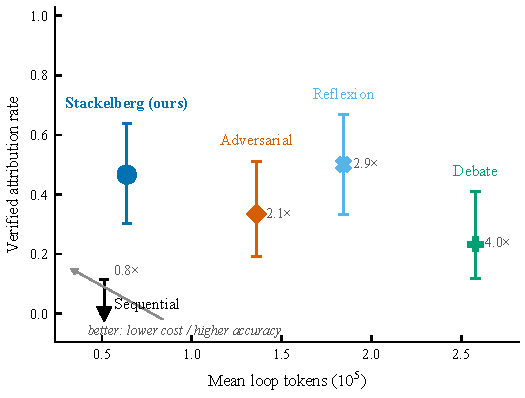
\includegraphics[width=0.55\linewidth]{fig4_exp_b_pareto.pdf}
\caption{Verified attribution versus mean loop-token cost across the five
Exp-B methods ($n{=}30$ shared frozen blackboards each; error bars:
Wilson 95\% CIs). Stackelberg sits on the efficient frontier at the
lowest token cost; adversarial trails its point estimate only
non-significantly at $2.1\times$ the cost, and the external multi-call
protocols cost $2.9\times$ (Reflexion) to $4.0\times$ (Debate).
Reflexion's higher point estimate ($0.50$ vs $0.47$) is not significant
--- its interval overlaps Stackelberg's over most of its range
($3{:}4$ discordant pairs, $p=1.0$).}
\label{fig:expb}
\end{figure}

\begin{table}[t]
\centering
\caption{Exp-B unified baselines --- \textbf{measured} (evidence-informed;
snapshot mode; $n{=}30$; $K{=}3$; shared frozen blackboards across all
methods; loop-token accounting). Primary: verified attribution.}
\label{tab:exp_baselines}
\label{tab:exp_ii}
\label{tab:exp_iii}
\begin{tabular}{@{}ll c c c c@{}}
\toprule
Family & Method & Verified attr.\ & First-probe & SSR@$K$ & Mean loop tokens \\
\midrule
Proposed & stackelberg (causal)
  & $14/30$ (0.47) & $30/30$ (1.00) & $21/30$ & $0.64{\times}10^{5}$ \\
Internal & adversarial
  & $10/30$ (0.33) & $19/30$ (0.63) & $13/30$ & $1.36{\times}10^{5}$ \\
Internal & sequential
  & $0/30$ (0.00) & $0/30$ (0.00) & $10/30$ & $0.51{\times}10^{5}$ \\
External & debate (3-voter panel)
  & $7/30$ (0.23) & $19/30$ (0.63) & $7/30$ & $2.58{\times}10^{5}$ \\
External & reflexion (memory critique)
  & $15/30$ (0.50) & $19/30$ (0.63) & $16/30$ & $1.84{\times}10^{5}$ \\
\bottomrule
\end{tabular}
\end{table}

\paragraph{Preliminary results (status-prior; real $n{=}5$, internal only).}
Table~\ref{tab:exp_baselines_prelim}: last-comply attribution was $0/5$ for
all three methods, while SSR diverged (sequential repaired $2/5$ blind,
stackelberg $1/5$, adversarial $0/5$). The attribution failure is uniform
across protocol families---single-judge accusation, committed causal
probing, blind reverse-chain repair---so no protocol's comply/deflect
responses identified the planted layer under last-comply accounting;
conversely, sequential's blind-repair SSR shows that eventual repair is
likewise uninformative about root cause. These two observations motivated
the verified attribution accounting and the evidence-informed rank of the
redesign. External baselines were not run in that preliminary pass.

\begin{table}[t]
\centering
\caption{Exp-B preliminary internal baselines (status-prior; real $n{=}5$).}
\label{tab:exp_baselines_prelim}
\label{tab:exp_ii_prelim}
\begin{tabular}{@{}l c c c c@{}}
\toprule
Method & Attr.\ hit & First-probe hit & SSR@$K$ & Mean tokens \\
\midrule
stackelberg (causal) & 0/5 (0.00) & 4/5 (0.80) & 1/5 & $1.38{\times}10^{5}$ \\
adversarial & 0/5 (0.00) & 2/5 (0.40) & 0/5 & $2.35{\times}10^{5}$ \\
sequential & 0/5 (0.00) & 0/4 (0.00) & 2/5 & $0.86{\times}10^{5}$ \\
\bottomrule
\end{tabular}
\end{table}

\subsection{Exp-C: Inspection diagnostics}
\label{sec:exp_diag}
\label{sec:exp_iv}

\paragraph{Question.}
Is commitment operational in the implementation---not merely additional LLM
calls? As the budget $K$ grows, does verified attribution rise under causal
commitment, and are inconsistent deflects overturned by executed refutation?

\paragraph{Design.}
We sweep $K$ for causal Stackelberg (and, as references, adversarial and
sequential) on the same injection grid, recording verified attribution versus
$K$, deflect rates, and the fraction of deflects/compliances overturned by
re-solve. Analysis-mode payoffs $(u_L,u_F)$ from Section~\ref{sec:payoff}
may be reported as secondary trajectory summaries.

\paragraph{Expected conclusion.}
Verified attribution rises with $K$ faster under causal Stackelberg than under
random/reverse or non-committed baselines; deflects that contradict re-solve
are overturned at high rate. Flat curves in $K$ or near-zero overturn rates
indicate that commitment is not operational.

\paragraph{Measured results (offline re-analysis of the completed grid).}
Table~\ref{tab:exp_diag} reports an offline reconstruction of per-probe
dynamics from the event logs of the smoke-grid campaigns above (seven
method arms, all on the same thirty frozen blackboards; re-analysis adds
no runs): verified-at-round-$k$ is read cumulatively within the completed
$K{=}3$ episodes, a comply is \emph{overturned} when the executed re-solve
re-enters diagnosis, and a deflect is \emph{false} when it comes from the
eventually verified layer. Three readings follow. First, the curves are
step functions positioned by where the guilty layer sits in the order:
under causal commitment all fourteen verified attributions occur at the
\emph{first} probe ($14/30$ at $K{=}1$, saturated --- the first-probe
confirmations of Section~\ref{sec:exp_metrics}), reverse reaches zero at
$K{=}1$ and its full $7/30$ only at $K{\ge}2$, and random lies between
($9$ hits at $K{=}1$, $12$ by $K{=}2$, $13$ at $K{=}3$). The
registered ``rises faster under causal'' clause thus holds in the
step-function sense, and the deeper diagnostic is that every method
\emph{except} random is flat from $K{=}2$ to $K{=}3$ (random's single
$K{=}3$ recovery is one more shuffle whose order reaches the guilty layer
only on the third probe): within this budget the operative variable is the
alignment of $\omega_1$ with $a^{\star}$, not budget depth (for the
non-Reflexion methods a $K{>}3$ sweep was not run; Reflexion was swept to
$K{=}5$ as the budget-tilted challenger of Section~\ref{sec:exp_baselines}
and gains nothing beyond round two). Second, deflects are near-truthful with
one qualified exception: across all $465$ recorded probes by the seven
methods --- the complete event-log population ($208$ of the $210$
episodes contribute probes; the remaining two crashed at the execution
stage before any probe) --- $116$ deflects were recorded, $113$ of them
from innocent downstream layers, and within the three committed order
arms the guilty layer complied at first contact on every board. The
exception is instructive: the only three guilty-layer deflections (two
Debate cells, one Reflexion cell) all occur \emph{after} the guilty
layer's round-one complying repair was overturned by the re-solve ---
late-stage re-accusation defences arguing that a passing solver status
leaves no error to own, not concealment of visible guilt. This is still
the truthful-best-response behaviour the commitment-plus-refutation
mechanism is designed to induce where it binds (single-plant caveat: the
model-layer plant's guilt is visible in its own output). Third, executed
refutation is load-bearing: $43$--$71\%$ of complies are overturned by
the re-solve (the repair claimed success but the objective did not
recover), so a comply is never taken on trust. Debate's $56\%$ deflect
rate is the panel's data-layer accusations being rejected by the data
layer's own backward check; Reflexion's $9\to15$ jump between $K{=}1$ and
$K{=}2$ reflects its memory-driven revision escaping bad first
attributions, consistent with its multi-round profile in the external
comparison. Figure~\ref{fig:expc} plots the step curves.

\begin{figure}[pos=htbp]
\centering
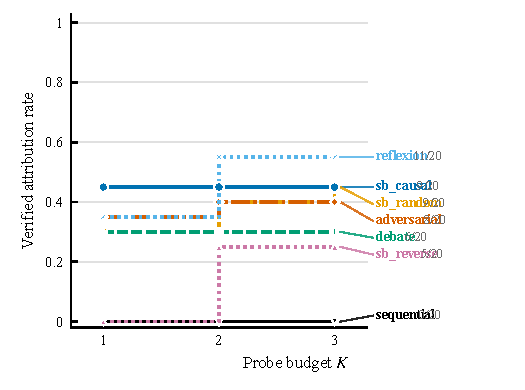
\includegraphics[width=0.6\linewidth]{fig3_exp_c_steps.pdf}
\caption{Verified attribution as a function of probe budget $K$ (Exp-C
offline re-analysis; $n{=}30$ shared blackboards per method; cumulative
within the completed $K{=}3$ episodes). The curves are step functions
positioned by the rank of the guilty layer in the committed order
$\omega$: causal commitment saturates at $K{=}1$ ($14/30$), reverse reaches
its plateau only at $K{\ge}2$, sequential never leaves zero, and
Reflexion's $9\to15$ jump between $K{=}1$ and $K{=}2$ reflects
memory-driven revision of bad first attributions. Every method except
random is flat from $K{=}2$ to $K{=}3$.}
\label{fig:expc}
\end{figure}

\begin{table}[t]
\centering
\caption{Exp-C diagnostics --- \textbf{measured} (offline re-analysis of
the completed smoke-grid episodes; $n{=}30$ shared blackboards per method;
verified attr.\ cumulative within the completed $K{=}3$ episodes).}
\label{tab:exp_diag}
\label{tab:exp_iv}
\begin{tabular}{@{}l c c c c c c@{}}
\toprule
Method & $K{=}1$ & $K{=}2$ & $K{=}3$ & Probes/cell & Deflect & Comply overturn \\
\midrule
stackelberg causal & $14/30$ & $14/30$ & $14/30$ & 1.8 & 26\% & 49\% \\
stackelberg random & $9/30$ & $12/30$ & $13/30$ & 2.1 & 32\% & 43\% \\
stackelberg reverse& $0/30$ & $7/30$ & $7/30$ & 2.2 & 22\% & 71\% \\
adversarial        & $8/30$ & $10/30$ & $10/30$ & 2.3 & 16\% & 60\% \\
sequential         & $0/30$ & $0/30$ & $0/30$ & 2.4 & 7\%  & 56\% \\
debate             & $7/30$ & $7/30$ & $7/30$ & 2.5 & 56\% & 64\% \\
reflexion          & $9/30$ & $15/30$& $15/30$& 2.2 & 14\% & 55\% \\
\bottomrule
\end{tabular}
\end{table}

\subsection{Failure-mode analysis}
\label{sec:exp_failure_modes}

Table-level rates do not reveal where the mechanism breaks, so we
additionally inspected the per-node event logs and repair artifacts of
every measured cell above and of the intervening single-run smokes. Three
recurrent failure families emerged; each is a property of the implemented
pipeline under layered faults, and each motivated a specific element of
the measured design or of the pending expanded grid.

\paragraph{Traceback-as-oracle.}
On crash surfaces the failure evidence points at the generated code, and
ranking that trusts the surface tips the code layer. Under an
intermediate evidence-informed variant with LLM-only ranking (same grid,
$n{=}3$), two of three causal cells committed a code-first $\omega$, spent
the budget on code- and data-layer overturns, and never reached the model
layer; verified attribution was $0/9$ over that grid. This is the
practical form of the symptom-locus ambiguity of
Section~\ref{sec:layered}: the traceback marks where the pipeline broke,
not where the defect was planted. The hybrid ranking of the measured
tables counters it with an explicit symptom-signature rule---a
forced-zero balance is model-layer evidence---while still ignoring
LLM-reported confidence.

\paragraph{Stale evidence at repair time.}
A correct tip does not guarantee a verified attribution: in that same
intermediate variant, the one cell that tipped the model layer still
failed, because its backward step consumed the pre-fault forward output,
in which the planted constraint was absent; the repair rewrote an
unrelated model element and was overturned by the re-solve. The measured
implementation presents the repairing agent with the current (post-fault)
output and restricts the repair to a minimal strip of the implicated
constraint rather than a free regeneration.

\paragraph{Residual repair-path variance.}
The measured campaigns retain a regeneration instability downstream of a
correct model-layer repair: a code-layer regeneration can fail outright
(in a single-run smoke it raised a key error and left a large objective
gap despite a correct strip); one sequential grid cell terminated before
any model call; and replicate variance remains high---the adversarial arm
reached a verified attribution in a single-run smoke but $0/3$ on the
grid. Success can also occur without attribution: seven causal cells
reached \emph{Practical Optimal} through a downstream repair while their
attributed layer settled on the code layer (the stolen-attribution branch
of the Exp-A confirmation funnel). These residuals concentrate in the paths
the deterministic data-layer contract now constrains; the no-plant gate
and the re-established tables of Section~\ref{sec:exp_reporting} bound
them before the expanded grid is interpreted, and the overturn and
deflect diagnostics of Exp.~\ref{sec:exp_diag} will quantify them at
scale.

\paragraph{Rank-invisible semantic faults.}
The Phase-4 data-layer plant exposes a fourth family. A contract-valid
semantic source swap leaves every structural signal intact---the validator
passes, the model formulates, the code runs---and the failure surface
(OPTIMAL with a gap) is indistinguishable from a modeling fault, so the
hybrid rank named the data layer first in $0$ of $10$ boards and causal
naming failed across the board (Table~\ref{tab:exp_multiplant}). Worse,
in $12$ of $22$ freeze attempts the swapped parameter never entered the
generated model at all and the run solved to the un-faulted optimum to
machine precision---a silent fault. Semantic data faults therefore
require evidence beyond the current surface smells (e.g., provenance
checks on which catalog table feeds which parameter), a design revision
registered for future work rather than patched post hoc.

\paragraph{Claim boundary.}
Comparisons are scoped to layered-error natural-language optimization on the
TSLP ECR pipeline. We do not claim gains for general LLM reasoning, nor that
inspection is the unique protocol that can eventually repair a failed solve.
The intended positive claim is that evidence-informed causal-order committed
inspection matches (or exceeds) strong single-judge naming accuracy while
improving verifiable attribution and auditability relative to unordered
commitment and to non-committed verification baselines under the injection
regime above. The visibility reading carries one further threat: each fault
layer is represented by a \emph{single} plant, so ``the model layer is
visible to the rank / the semantic data layer is not'' is established for
the tested plant families, not for layers as such --- a different model-layer
plant without a symptom signature could be as rank-invisible as the
semantic swap. Within-layer plant replication is therefore registered
alongside the data-layer evidence revision before the visibility claim is
read as a layer property.

%==============================================================================
\section{Conclusion}
\label{sec:conclusion}

We recast diagnosis--repair in an LLM optimization pipeline as a
Stackelberg inspection game and asked what the inspector's commitment
is actually worth. The empirical answer, across three fault plants,
three problem instances, five diagnosis protocols, and the $465$ probe
rounds recorded across the seven arms of the shared grid, is precise
about the mechanism:
\emph{committed alignment carries the information}. Probing is bound to
the committed order --- the executed first probe equals $\omega_1$ on
every board ever run --- so first-probe naming is exactly the ranking's
alignment, and the ranking sees the model layer (through
symptom signatures) and the code layer (through relaxed-solve surfaces)
but not contract-valid semantic data faults, for which naming failed for
every fixed order. Naming is not confirmation: on the main grid only
$14$ of the $30$ aligned first probes are settled by the round-one
re-solve ($9$ overturned repairs, $7$ attributions stolen by downstream
regeneration), while on the reverse arm $8$ misaligned probes absorbed
the upstream fault outright and succeeded without verified attribution.
The order-effect claim is therefore conditionally
replicated, not universal, and we register the corresponding design
revision (provenance-style evidence for the data layer) rather than
patching it post hoc.

The quantitative picture is consistent with that mechanism. On the
shared frozen blackboards of the main grid, causal Stackelberg names
the guilty layer with its first probe on every board and dominates single-judge,
debate, and reflexion naming ($11{:}0$ discordant pairs each); verified
attribution reaches $0.60$ versus $0.20$ under reverse commitment on the
instance family (pooled paired $p=0.008$) and $0.47$ versus $0.23$ on the
densified main grid ($8{:}1$, $p=0.039$); and the budget diagnostics
show that nothing improves after the second round within the budgets
tested ($K{=}3$ for all arms; $K{=}5$ for Reflexion as the tilted
challenger) ---
the guilty layer's position, not budget depth, is what the curves
respond to. On the single tested engine, external multi-call protocols
do not overturn the design: debate and reflexion name no better than one
judge, debate's verified attribution is significantly lower
($8{:}1$, $p=0.039$) at $4.0\times$ the loop tokens, and reflexion's
non-significant verified edge ($0.50$ versus
$0.47$) costs $2.9\times$ the loop tokens without a committed order or
its audit trail. Two
mechanism checks close the loop between theory and logs: under
commitment the guilty layer complied at first contact on every
committed-arm board (the three deflections observed, all in external
arms, follow an overturned repair), while $43$--$71\%$ of complying
repairs were overturned by the re-solve --- verification, not cheap
talk, is what carries attribution.

The claims are bounded accordingly: the first-contact-compliance result
is established on the model-layer plant (whose guilt is visible in its own
output; the three guilty-layer deflections observed, all in external
arms, follow an overturned repair) and is silent on the semantic data
plant, whose $55\%$
silent-fault rate means most injected faults never produced a failure
board and deflect behaviour was never exercised; the instance family
varies horizon and scenario count at fixed network size, the main
campaigns run a single engine under a frozen implementation (the
second-engine spot-check covers five boards), $K$ is capped at three
(five for the Reflexion challenger), and each fault layer is represented
by one plant, so visibility is a property of the tested plant families
rather than of layers as such. Within those bounds the
contribution stands as a mechanism, a proposition with matching
dynamics, and a measured protocol: commitment buys naming accuracy and
cheaper verifiable attribution precisely when the committed ranking can
see the fault --- and the logs show why. Extending visibility to the
semantic data layer, replicating within layers across additional plants,
scaling the network, and a full cross-engine
campaign (a second-engine spot-check already replicates the
commitment-side alignment structure with zero exceptions) are the
registered next steps.

%==============================================================================
\section*{Data and code availability}
The frozen instance data, fault-injection plants, run manifests, and
per-node event logs supporting every measured table, together with the
pipeline implementation, will be released upon acceptance.

%==============================================================================
\begin{thebibliography}{99}
\bibitem[Wu et al.(2024)]{wu2024autogen} Q.~Wu et al. AutoGen: Enabling next-gen LLM applications via multi-agent conversation. In \emph{COLM}, 2024.
\bibitem[Xiao et al.(2024)]{xiao2023coe} Y.~Xiao et al. Chain-of-experts: When LLMs meet complex operations research problems. In \emph{ICLR}, 2024. \url{https://openreview.net/forum?id=HobyL1B9CZ}.
\bibitem[AhmadiTeshnizi et al.(2024a)]{ahmaditeshnizi2024optimus} A.~AhmadiTeshnizi, W.~Gao, M.~Udell. OptiMUS: Scalable optimization modeling with (MI)LP solvers and large language models. In \emph{ICML}, PMLR 235:577--596, 2024. \url{https://arxiv.org/abs/2402.10172}.
\bibitem[AhmadiTeshnizi et al.(2024b)]{ahmaditeshnizi2024optimus03} A.~AhmadiTeshnizi, W.~Gao, H.~Brunborg, S.~Talaei, M.~Udell. OptiMUS-0.3: Using large language models to model and solve optimization problems at scale. \emph{arXiv:2407.19633}, 2024.
\bibitem[Yang et al.(2025)]{yang2025orthought} B.~Yang, Q.~Zhou, J.~Li, C.~Su, P.~Angeloudis, S.~Hu. ORThought: Benchmarking and automating logistics optimization modeling via structured LLM reasoning. \emph{arXiv:2508.14410}, 2025.
\bibitem[Du et al.(2023)]{du2023improving} Y.~Du, S.~Li, A.~Torralba, J.~B.~Tenenbaum, I.~Mordatch. Improving factuality and reasoning in language models through multiagent debate. \emph{arXiv:2305.14325}, 2023.
\bibitem[Liang et al.(2024)]{liang2024mad} T.~Liang, Z.~He, W.~Jiao, et al. Encouraging divergent thinking in large language models through multi-agent debate. In \emph{EMNLP}, pages 17889--17904, 2024.
\bibitem[Shinn et al.(2023)]{shinn2023reflexion} N.~Shinn, F.~Cassano, A.~Gopinath, K.~Narasimhan, S.~Yao. Reflexion: Language agents with verbal reinforcement learning. In \emph{NeurIPS}, 2023.
\bibitem[Zhang et al.(2025)]{zhang2025whowhen} S.~Zhang, M.~Yin, J.~Zhang, et al. Which agent causes task failures and when? On automated failure attribution of LLM multi-agent systems. In \emph{ICML}, PMLR 267:76583--76599, 2025. \url{https://arxiv.org/abs/2505.00212}.
\bibitem[Chen et al.(2026)]{chen2026traceelephant} M.~Chen, J.~Wang, F.~Mu, et al. Seeing the whole elephant: A benchmark for failure attribution in LLM-based multi-agent systems. In \emph{ACL}, 2026. \url{https://arxiv.org/abs/2604.22708}.
\bibitem[Wang et al.(2026)]{wang2026chief} Y.~Wang, W.~Wu, J.~Wang, Q.~Wang. From flat logs to causal graphs: Hierarchical failure attribution for LLM-based multi-agent systems. \emph{arXiv:2602.23701}, 2026.
\bibitem[Shah(2026)]{shah2026car} J.~Shah. Causal Agent Replay: Counterfactual attribution for LLM-agent failures. \emph{arXiv:2606.08275}, 2026.
\bibitem[Yi et al.(2025)]{yi2025econ} X.~Yi, Z.~Zhou, C.~Cao, Q.~Niu, et al. From debate to equilibrium: Belief-driven multi-agent LLM reasoning via Bayesian Nash equilibrium. In \emph{ICML}, 2025. \url{https://proceedings.mlr.press/v267/yi25c.html}.
\bibitem[Wang(2026)]{stackelberg2026resource} B.~Wang. A Stackelberg framework for resource-aware LLM agents: Learning, repair, and conditional guarantees. \emph{arXiv:2606.23026}, 2026.
\bibitem[von Stackelberg(1952)]{stackelberg1952} H.~von~Stackelberg. \emph{The Theory of the Market Economy}. Oxford University Press, 1952.
\bibitem[Avenhaus et al.(2002)]{avenhaus2002inspection} R.~Avenhaus, B.~von~Stengel, S.~Zamir. Inspection games. In R.~J.~Aumann and S.~Hart (eds.), \emph{Handbook of Game Theory with Economic Applications}, vol.~3, ch.~51, pp.~1947--1987. Elsevier, 2002.
\bibitem[Maschler(1966)]{maschler1966inspection} M.~Maschler. A price leadership method for solving the inspector's non-constant-sum game. \emph{Naval Research Logistics Quarterly}, 13(1):11--33, 1966.
\bibitem[Korzhyk et al.(2011)]{korzhyk2011security} D.~Korzhyk, Z.~Yin, C.~Kiekintveld, V.~Conitzer, M.~Tambe. Stackelberg vs.\ Nash in security games: An extended investigation of interchangeability, equivalence, and uniqueness. \emph{Journal of Artificial Intelligence Research}, 41:297--327, 2011. \url{https://doi.org/10.1613/jair.3269}.
\bibitem[Tambe(2011)]{tambe2011security} M.~Tambe. \emph{Security and Game Theory: Algorithms, Deployed Systems, Lessons Learned}. Cambridge University Press, 2011.
\bibitem[Poiani et al.(2024)]{poiani2024ecr} R.~Poiani, C.~Stirbu, A.~M.~Metelli, M.~Restelli. Optimizing empty container repositioning and fleet deployment via configurable Semi-POMDPs. \emph{IEEE Transactions on Intelligent Transportation Systems}, 25(5):4704--4711, 2024. \url{https://doi.org/10.1109/TITS.2023.3329677}.
\bibitem[Wang et al.(2025a)]{wang2025ecrslot} W.~Wang, C.~Diao, W.~He, Z.~Jin, Z.~Yang. Collaborative optimization of container liner slot allocation and empty container repositioning within port clusters. \emph{Journal of Marine Science and Engineering}, 13(1):159, 2025. \url{https://doi.org/10.3390/jmse13010159}.
\bibitem[Cai et al.(2025)]{cai2025ecrjoint} J.~Cai, Y.~Huang, C.~Diao, Z.~Jin. Joint optimization of multi-period empty container repositioning and inventory control based on adaptive particle swarm algorithm. \emph{Journal of Marine Science and Engineering}, 13(6):1113, 2025. \url{https://doi.org/10.3390/jmse13061113}.
\bibitem[Liu et al.(2025)]{liu2025llmtransport} T.~Liu, J.~Yang, Y.~Yin. Toward LLM-agent-based modeling of transportation systems: A conceptual framework. \emph{Artificial Intelligence for Transportation}, 1:100001, 2025. \url{https://doi.org/10.1016/j.ait.2025.100001}.
\end{thebibliography}

\end{document}
